% !TeX program = pdflatex
% !TeX encoding = UTF-8
% OVERLEAF: selecione artigo.tex como documento principal; compilador pdfLaTeX.
% Exige as imagens da pasta figuras/. Não usa arquivos .bib nem estilos locais.
%
% Normas de referência:
% - ABNT NBR 6022:2018: estrutura e apresentação de artigos científicos.
% - ABNT NBR 6024:2012: numeração progressiva das seções.
% - ABNT NBR 6028:2021: resumos e palavras-chave.
% - ABNT NBR 10520:2023: citações.
% - ABNT NBR 6023:2025: referências.
%
% A NBR 6022 permite que o periódico defina seu projeto gráfico. Sem um
% modelo institucional específico, adotam-se A4, fonte Times de 12 pontos,
% margens superior/esquerda de 3 cm e inferior/direita de 2 cm.
% A entrelinha simples segue a recomendação para artigos da NBR 6022.
% Fontes para consulta:
% https://ctan.org/pkg/abntex2
% https://biblioteca.ufes.br/normalizacao

\documentclass[
  article,
  12pt,
  oneside,
  a4paper,
  english,
  brazil
]{abntex2}

% Codificação, fonte com suporte a acentos e recursos básicos.
\usepackage[T1]{fontenc}
\usepackage[utf8]{inputenc}
\usepackage{newtxtext}
\usepackage{newtxmath}
\usepackage{microtype}
\usepackage{graphicx}
\usepackage{booktabs}

% Margens e parágrafos.
\setlrmarginsandblock{3cm}{2cm}{*}
\setulmarginsandblock{3cm}{2cm}{*}
\checkandfixthelayout
\SingleSpacing
% Caso a instituição exija entrelinha 1,5, substitua a linha anterior por:
% \OnehalfSpacing
\setlength{\parindent}{1.25cm}
\setlength{\parskip}{0pt}
\frenchspacing

% Seções alinhadas à esquerda, com hierarquia tipográfica e fonte 12.
\setsecheadstyle{\normalfont\normalsize\bfseries\raggedright\MakeTextUppercase}
\setsubsecheadstyle{\normalfont\normalsize\bfseries\raggedright}
\setsubsubsecheadstyle{\normalfont\normalsize\itshape\raggedright}
\setsecnumdepth{subsubsection}
\setbeforesecskip{\baselineskip}
\setaftersecskip{\baselineskip}
\setbeforesubsecskip{\baselineskip}
\setaftersubsecskip{\baselineskip}

% Fonte menor uniforme para notas, legendas e citações longas.
\renewcommand{\ABNTEXfontereduzida}{\fontsize{10}{12}\selectfont}
\setlength{\ABNTEXcitacaorecuo}{4cm}
\captionnamefont{\ABNTEXfontereduzida}
\captiontitlefont{\ABNTEXfontereduzida}
\captionstyle{\raggedright}

% Paginação no canto superior direito, sem cabeçalhos textuais.
\makepagestyle{artigo}
\makeoddhead{artigo}{}{}{\ABNTEXfontereduzida\thepage}
\makeoddfoot{artigo}{}{}{}
\aliaspagestyle{plain}{artigo}

% Elementos sem indicativo numérico, centralizados.
\newcommand{\secaosemnumero}[1]{%
  \par\addvspace{\baselineskip}%
  \phantomsection
  \pdfbookmark[1]{#1}{elemento-\thebookmarkelemento}%
  \stepcounter{bookmarkelemento}%
  {\centering\normalfont\normalsize\bfseries #1\par}%
  \nobreak\vspace{\baselineskip}}
\newcounter{bookmarkelemento}

% Dados do artigo: substituir os campos entre colchetes.
% Título provisório. Ajustar depois dos resultados da campanha.
\titulo{Custo do TreeSHAP em um sistema de detecção de intrusão em rede:
  estratégias de explicação, latência e cobertura}
\tituloestrangeiro{The cost of TreeSHAP in a network intrusion detection system:
  explanation strategies, latency and coverage}
\autor{Pedro Felipe Sousa Garcia\thanks{Graduando do Curso de Tecnologia em Análise e
  Desenvolvimento de Sistemas. Faculdade de Tecnologia de São José dos Campos: Professor Jessen
  Vidal (FATEC). São José dos Campos, Brasil.
  E-mail: \texttt{[TODO: e-mail]}.}
  \and
  José Walmir Gonçalves Duque\thanks{Mestre. Orientador. Faculdade de Tecnologia de São José dos
  Campos: Professor Jessen Vidal (FATEC). São José dos Campos, Brasil.}}
\data{}

\pretitle{\begin{center}\normalfont\normalsize\bfseries}
\posttitle{\par\end{center}}
\renewcommand{\maketitlehookb}{%
  \begin{center}\normalfont\normalsize\itshape
    \imprimirtituloestrangeiro
  \end{center}}

\hypersetup{
  hidelinks,
  pdftitle={Custo do TreeSHAP em um sistema de detecção de intrusão em rede},
  pdfauthor={Pedro Felipe Sousa Garcia; José Walmir Gonçalves Duque},
  pdfsubject={Artigo científico}
}

\begin{document}
\selectlanguage{brazil}
\maketitle
\pagestyle{artigo}
\thispagestyle{artigo}

\begin{center}
  \ABNTEXfontereduzida
  Submetido em: [dia/mês/ano]. Aprovado em: [dia/mês/ano].
\end{center}

% Roteiro do argumento (rascunho, a revisar depois dos resultados):
% 1. Um NIDS com aprendizado de máquina precisa classificar cada fluxo em pouco tempo, e quem analisa
%    um alerta precisa saber por que o fluxo foi classificado como ataque.
% 2. O TreeSHAP calcula essas explicações em tempo polinomial para modelos de árvores, mas acrescenta
%    a cada fluxo um cálculo de custo comparável ao da própria inferência.
% 3. Poucos trabalhos medem esse custo dentro do sistema, e quase nenhum compara, sob carga
%    controlada, formas diferentes de entregar as explicações.
% 4. O artigo pergunta se é viável explicar no momento da classificação sem violar restrições de
%    latência, comparando quatro estratégias de explicação.
% 5. Os dados, os classificadores e o explicador ficam fixos antes da campanha.
% 6. O NIDS de referência forma os mesmos fluxos que geraram os dados de treino e marca cinco
%    instantes por fluxo.
% 7. A carga cresce pela sobreposição de cópias do mesmo trecho, que preservam as entradas de cada
%    fluxo, ao contrário da reprodução acelerada.
% 8. Os resultados medidos até aqui mostram a qualidade da detecção, o custo isolado do TreeSHAP
%    e a validade do ambiente emulado.
% 9. A campanha mostra a latência, a cobertura e os recursos de cada estratégia sob cada carga.
% 10. A discussão relaciona os resultados com a pergunta e com os limites do ambiente.

\secaosemnumero{Resumo}
\noindent
Sistemas de detecção de intrusão em rede baseados em aprendizado de máquina classificam fluxos de
tráfego, mas suas decisões são difíceis de interpretar. O TreeSHAP explica cada classificação de
modelos de árvores pela contribuição de cada atributo, ao custo de um cálculo adicional por fluxo.
Este artigo mede esse custo num sistema de detecção de intrusão em rede (NIDS) com Random Forest e
XGBoost, treinados com o Improved CIC-IDS2017, e compara quatro estratégias de explicação: sem
explicação, síncrona total, síncrona condicional e assíncrona. O NIDS forma os mesmos fluxos dos
dados de treino, marca o instante de cada etapa de cada fluxo e roda numa rede emulada pelo Mininet.
A carga cresce com cópias simultâneas de um trecho de captura, cada uma com endereços próprios, o que
preserva as entradas dos fluxos. Em chamadas isoladas, a explicação de um fluxo
levou em média 7,4~ms no Random Forest e 0,43~ms no XGBoost, contra 4,9~ms e 0,18~ms da inferência.
Com 1, 2 e 4 cópias, o XGBoost manteve a latência de classificação abaixo
de 1~s no p95 e de 2~s no p99 em todas as estratégias, inclusive explicando todos os fluxos antes da
entrega, salvo numa execução com perda de pacotes. No Random Forest, explicar todos os fluxos só foi
viável na estratégia assíncrona com 1 cópia. A estratégia condicional não acrescentou latência
mensurável, mas explicou no máximo 2,8\% dos fluxos. A viabilidade depende do custo do TreeSHAP no
classificador e da carga.

\smallskip
\noindent\textbf{Palavras-chave:} detecção de intrusão; inteligência artificial explicável;
TreeSHAP; latência; CIC-IDS2017.

\begin{otherlanguage*}{english}
\secaosemnumero{Abstract}
\noindent
Machine learning-based network intrusion detection systems classify traffic flows, but their
decisions are hard to interpret. TreeSHAP explains each classification of tree-based models by the
contribution of each feature, at the cost of an additional computation per flow. This article measures
this cost in a network intrusion detection system (NIDS) with Random Forest and XGBoost, trained on
Improved CIC-IDS2017, and compares four explanation strategies: no explanation, fully synchronous,
conditional synchronous and asynchronous. The NIDS builds the same flows as the training data,
records the instant of each stage of each flow and runs on a network emulated with Mininet. The load
grows with simultaneous copies of a capture segment, each with its own addresses, which preserves
the flow inputs. In isolated calls, explaining one flow took on average 7.4~ms with Random Forest
and 0.43~ms with XGBoost, against 4.9~ms and 0.18~ms for inference. With 1, 2 and 4 copies, XGBoost
kept the p95 classification latency below 1~s and the p99 below 2~s under all strategies, including
when explaining every flow before delivery, except in one run with packet loss. With Random Forest,
explaining every flow was feasible only with the asynchronous strategy and 1 copy. The conditional
strategy added no measurable latency, but explained at most 2.8\% of the flows. Feasibility depends
on the load and on the cost of TreeSHAP for the classifier.

\smallskip
\noindent\textbf{Keywords:} intrusion detection; explainable artificial intelligence; TreeSHAP;
latency; CIC-IDS2017.
\end{otherlanguage*}

\textual
\pagestyle{artigo}

\section{Introdução}
\label{sec:introducao}

Um sistema de detecção de intrusão em rede (NIDS) procura ameaças no tráfego de uma rede e emite
alertas quando o tráfego casa com a assinatura de um ataque conhecido ou foge do comportamento
normal (Zuech; Khoshgoftaar; Wald, 2015). Num NIDS baseado em aprendizado de máquina, os pacotes podem ser
agrupados em fluxos, cada fluxo descrito por atributos como duração, tamanho dos pacotes e intervalo
entre eles, e cada fluxo classificado por um modelo treinado em tráfego rotulado. É o caso do
CIC-IDS2017, que descreve cada fluxo por 80 atributos e avalia sete algoritmos de aprendizado de
máquina sobre eles (Sharafaldin; Habibi Lashkari; Ghorbani, 2018). Modelos de árvores, como o
Random Forest (Breiman, 2001) e o XGBoost (Chen; Guestrin, 2016), têm bom desempenho em dados
tabulares como esses. No CIC-IDS2017, o ID3 e o Random Forest tiveram os dois maiores valores de F1
entre os sete algoritmos avaliados, 0,98 e 0,97 (Sharafaldin; Habibi Lashkari; Ghorbani, 2018). Em
comparações com vários conjuntos tabulares, o XGBoost superou modelos profundos recentes propostos
para esse tipo de dado e exigiu menos ajuste (Shwartz-Ziv; Armon, 2022), e os modelos de árvores
continuaram à frente das redes neurais profundas em conjuntos de cerca de 10 mil amostras
(Grinsztajn; Oyallon; Varoquaux, 2022). O Random Forest e o XGBoost combinam muitas árvores de
decisão, e, em modelos com muitas árvores, relatar o caminho de decisão de uma previsão não ajuda a
explicá-la (Lundberg et al., 2020). Num sistema de detecção de intrusão, a opacidade do modelo
dificulta ao analista de segurança validar alertas, investigar falsos positivos e entender
detecções perdidas, como observam Ogunseyi et al. (2026) para modelos de aprendizado profundo.

A inteligência artificial explicável (XAI) reúne técnicas que explicam as decisões de um modelo
(Adadi; Berrada, 2018). O TreeSHAP calcula, para cada previsão de um modelo de árvores, a contribuição de cada atributo, e a
soma das contribuições com um valor de referência reproduz a saída explicada. O método reduz o
cálculo exato dos valores de Shapley de tempo exponencial para tempo polinomial no número de folhas
e na profundidade das árvores (Lundberg et al., 2020). Mesmo polinomial, esse cálculo é uma segunda
operação por fluxo, ao lado da inferência. Num NIDS, ele pode atrasar a entrega da classificação,
encher filas e, em carga alta, fazer o sistema descartar fluxos.

A literatura mede pouco esse custo. Segundo a revisão sistemática de Ogunseyi et al. (2026), dos
129 estudos de detecção de intrusão com aprendizado profundo explicável analisados, apenas 12
relatam alguma métrica de eficiência, e nenhum compara quantitativamente a latência antes e depois
da explicação.
Dash e Acken (2026) definem a latência de detecção de ponta a ponta como a soma de três
componentes, sem incluir a explicação. Nugraha, Jnanashree e Bauschert (2025) explicam cada
decisão de um detector XGBoost com SHAP e LIME e medem o tempo de geração das explicações.
Le et al. (2026) propõem um mecanismo que escolhe entre sete ações de explicação sob restrição de
recursos e o comparam com políticas de limiar, e
Tolay (2026) mede o TreeSHAP em lotes e projeta o custo de explicar só parte das previsões.
Nenhum desses trabalhos mede, num NIDS sob carga controlada, a latência da classificação e a da
explicação de cada fluxo em estratégias de entrega diferentes.

Este artigo pergunta se é viável gerar explicações TreeSHAP no momento da classificação, num NIDS
baseado em aprendizado de máquina, sem violar as restrições de latência do tráfego. A hipótese é
que a explicação acrescenta um custo que varia com a estratégia e com a carga, e que explicar só
alguns fluxos ou explicar fora do caminho da classificação reduz esse custo, com compromissos
diferentes entre latência, uso de recursos e cobertura explicativa. Para testá-la, o trabalho
compara quatro estratégias de explicação num NIDS com Random Forest e XGBoost, numa rede emulada,
sob níveis de carga controlados.

O trabalho contribui com a medição dessas quatro estratégias num mesmo NIDS, com o mesmo caminho de
classificação, e com um ambiente em que a carga cresce sem alterar os atributos dos fluxos. A
Seção~\ref{sec:fundamentacao} apresenta o TreeSHAP, as medidas de latência e os trabalhos
relacionados. A Seção~\ref{sec:metodologia} descreve os dados, os classificadores, o NIDS, as
estratégias, o ambiente emulado e as medições. A Seção~\ref{sec:resultados} apresenta e discute os
resultados, e a Seção~\ref{sec:conclusao} responde à pergunta nos limites do experimento.

\section{Fundamentação teórica}
\label{sec:fundamentacao}

\subsection{Detecção de intrusão por fluxos}

O CIC-IDS2017 reúne cinco dias de tráfego de uma rede de laboratório, com tráfego benigno gerado a
partir do comportamento de usuários e ataques de sete famílias (Sharafaldin; Habibi Lashkari; Ghorbani,
2018). Os fluxos do conjunto e seus atributos vêm do CICFlowMeter, um extrator de atributos de
fluxos distribuído pelo mesmo instituto que criou o conjunto. Ele lê os pacotes de uma captura em
formato PCAP, agrupa num fluxo os pacotes com os mesmos endereços, portas e protocolo e calcula 80
atributos de cada fluxo, como a duração, os intervalos entre pacotes e as estatísticas de cada
sentido da comunicação (Sharafaldin; Habibi Lashkari; Ghorbani, 2018). Engelen, Rimmer e Joosen (2021) encontraram
erros na geração do tráfego, na formação dos fluxos, na extração de atributos e na rotulagem do
conjunto. Eles corrigiram o extrator, refizeram a extração e marcaram como \emph{Attempted} os
fluxos de ataque que não exibem comportamento malicioso. Liu et al. (2022) fizeram novas correções
no extrator e publicaram a versão usada neste trabalho, o Improved CIC-IDS2017.

Um fluxo agrega os pacotes trocados entre duas pontas, identificadas por endereço, porta e
protocolo, até que uma regra do extrator o encerre (Engelen, 2022). No CICFlowMeter corrigido, um fluxo termina por
tempo limite, por um encerramento TCP seguido de uma nova conexão, por um pacote ICMP com código e
tipo diferentes dos do fluxo ou no fim da captura (Engelen, 2022). Esse modo de
encerramento importa para a latência. Um NIDS que usa os mesmos atributos do treino só pode
classificar um fluxo depois que o fluxo termina, o que pode levar até o tempo limite de 120~s
depois do primeiro pacote (Engelen, 2022).

\subsection{Valores de Shapley e TreeSHAP}

Os valores de Shapley vêm da teoria dos jogos cooperativos e repartem o resultado de um jogo entre
os jogadores pela contribuição marginal média de cada um (Shapley, 1953). Aplicados a uma previsão, os jogadores são
os atributos, e o resultado é a saída do modelo para a entrada explicada (Lundberg et al., 2020). Lundberg e Lee
(2017) mostram que, entre os métodos de atribuição aditiva, os valores de Shapley são
os únicos que satisfazem três propriedades: a precisão local, pela qual as atribuições somadas ao
valor de referência reproduzem a saída explicada, a consistência e a ausência de efeito de atributos
ausentes.

O cálculo exato desses valores é exponencial no número de atributos. Para árvores, o TreeSHAP o
reduz a $O(TLD^2)$, em que $T$ é o número de árvores, $L$ o maior número de folhas e $D$ a maior
profundidade (Lundberg et al., 2020). Na variante \emph{path-dependent}, a ausência de um atributo é
representada pela proporção de registros de treino que seguem cada ramo, guardada no próprio modelo
como a cobertura de cada nó, e o cálculo dispensa um conjunto de referência (Lundberg et al.,
2020). Na variante
\emph{interventional}, a ausência é representada por um conjunto de referência, e o custo cresce
com o tamanho desse conjunto (Lundberg et al., 2020).

\subsection{Latência num NIDS}

Dash e Acken (2026) tratam a latência de detecção como a rapidez com que um sistema de detecção de
intrusão identifica as intrusões. Eles observam que os trabalhos da área a definem de modos
diferentes, como tempo de inferência, de comunicação ou de computação, o que torna os resultados
incomparáveis. A definição que propõem soma três componentes, a latência controlada pelo atacante,
a latência determinada pelo sistema de detecção e a latência posterior à detecção, e decompõe a
segunda em componentes que dependem da topologia da rede e do método de detecção.
Este trabalho mede três tempos por fluxo. O tempo de inferência é a duração da chamada ao
classificador. A latência de classificação vai do fim da extração dos atributos do fluxo ao momento
em que a classificação fica disponível a quem a consome. A latência de explicação vai do mesmo
início ao momento em que a explicação fica disponível. A diferença entre a latência de
classificação de uma estratégia e a da classificação sem explicação, sob a mesma carga e o mesmo
classificador, é a sobrecarga de latência da estratégia.

\subsection{Trabalhos relacionados}

Bertoli et al. (2020) mostram que o desempenho de um detector medido no sistema em funcionamento
difere do medido sobre o conjunto de dados. Eles treinaram uma árvore de decisão sobre 12 atributos
do cabeçalho TCP/IP para detectar varreduras TCP e a implementaram como módulo do núcleo do Linux num
Raspberry Pi, com o tráfego de ataque passando pelo sistema. A árvore de profundidade 11, com F1 de
0,96 na análise do conjunto de dados, teve acurácia de 68\% nos ataques avaliados no sistema. A de
profundidade 6, com F1 de 0,92, teve 82\%. Este trabalho adota a mesma avaliação de ponta a ponta
para medir o custo das explicações, que aquele trabalho não trata.

Nugraha, Jnanashree e Bauschert (2025) propõem um arcabouço de detecção explicável em duas etapas. A
primeira combina um teste estatístico com os valores SHAP globais para manter os dez atributos mais
informativos, e a segunda treina um detector XGBoost e explica cada decisão com SHAP e LIME,
comparando as duas explicações. A avaliação usa três conjuntos de dados, entre eles o CICIoT2023, e
mede o tempo de geração das explicações, que no LIME caiu de 36~s para 4,9~s com o arcabouço.

Le et al. (2026) tratam a explicação como um serviço com custo num NIDS com recursos limitados. O
mecanismo que propõem escolhe entre sete ações de explicação, como suprimir, adiar, gerar a
explicação local completa ou transferi-la para outro nível da rede, conforme a pressão de pacotes, a
dívida de explicações e um orçamento de exposição do modelo. A avaliação usa processos de chegada
sintéticos ou reproduzidos e sequências de escores calibradas em três conjuntos de dados, e o custo
de cada ação é um peso normalizado, e não uma latência medida. No regime em que um adversário infla a
demanda por explicações, o mecanismo reduziu a dívida média de explicações em 57,3\% em relação a
políticas de limiar.

Tolay (2026) mede o tempo do TreeSHAP em Random Forest e XGBoost treinados no CICIoT2023, em lotes
de 1 a 5.000 registros, num computador com processador Intel Core 7 240H, e projeta a economia de
explicar só parte das previsões. A política que explica os ataques previstos e os benignos acima de
um limiar economiza mais quando os ataques são raros. Os tempos medem a chamada do explicador, fora
de um sistema que recebe tráfego.

Entre esses trabalhos, o que mede o custo do TreeSHAP mede a chamada do explicador, e o que trata a
explicação como serviço sob carga usa custos simulados. Este trabalho mede, num mesmo NIDS e com o
mesmo caminho de classificação, a latência da classificação e a da explicação de cada fluxo nas
quatro estratégias, numa rede emulada em que a carga cresce sem alterar os atributos dos fluxos.

\section{Metodologia}
\label{sec:metodologia}

\subsection{Dados e rótulos}

Os dados de treino são os cinco arquivos diários do Improved CIC-IDS2017 (Liu et al., 2022), com
2.099.976 registros de fluxo. A classificação é binária. Os fluxos com rótulo \emph{BENIGN} e os
fluxos \emph{Attempted}, que não exibem comportamento malicioso, são benignos, e os demais são
ataques, o que dá 1.594.545 registros benignos (75,93\%) e 505.431 de ataque (24,07\%). O
classificador recebe 80 atributos de cada fluxo. Os endereços, as portas e o instante do fluxo
ficam fora das entradas, para que o modelo não aprenda as máquinas e os horários do laboratório em
que o conjunto foi gerado. Os dois comprimentos de cabeçalho também ficam fora. O extrator os calcula em inteiros de 64 bits
(Engelen, 2022), mas a rotulagem do dataset os gravou em inteiros de 16 bits (Engelen, 2023). Acima
de 32.767, o valor gravado dá a volta e passa a diferir do que o extrator calcula em operação. Nos dois atributos de taxa, o valor infinito é
substituído por $-1$.

Os registros são divididos em 70\% para treino, 15\% para validação e 15\% para teste. A divisão
agrupa os registros com as 80 entradas idênticas e coloca cada grupo inteiro em um único conjunto,
porque 447.899 registros (21,33\%) pertencem a 63.136 grupos de entradas repetidas, e uma divisão
por registro poria cópias do treino no teste. A divisão é estratificada pelos 27 rótulos originais,
com semente fixa. O treino ajusta os classificadores, a validação escolhe as configurações e
calibra os critérios de seleção, e o teste só é usado na avaliação final da detecção.

\subsection{Classificadores}

O Random Forest e o XGBoost foram escolhidos entre três configurações cada, pelo maior F1 na
validação, com treino numa amostra de 100 mil registros. O Random Forest usa 100 árvores com
profundidade máxima de 12 e no mínimo dois registros por folha. O XGBoost usa 100 árvores com
profundidade máxima de 6 e taxa de aprendizagem de 0,1, com objetivo logístico binário. As
configurações escolhidas foram treinadas com os 1.469.983 registros do treino e congeladas antes da
abertura do teste. Um fluxo é classificado como ataque quando a probabilidade de ataque passa de
0,5. Carregados em processos novos, os dois modelos congelados reproduziram todas as classificações
dos 314.993 registros do teste.

\subsection{Explicações}

O TreeSHAP usa a variante \emph{path-dependent}, sem conjunto de referência, na biblioteca
\texttt{shap} 0.54.1. O tamanho de um conjunto de referência seria um parâmetro a mais, e o custo da
variante \emph{interventional} cresce com ele (Lundberg et al., 2020). No Random Forest, a saída
explicada é a probabilidade de ataque. No XGBoost, é o escore anterior à função logística, na escala
de log-odds, porque a variante \emph{path-dependent} só explica a saída bruta das árvores (Shap, 2026). As
contribuições dos dois classificadores ficam, assim, em escalas diferentes. As implementações
também diferem. No Random Forest, o cálculo é feito pela extensão em C do \texttt{shap}, e no
XGBoost, pelo TreeSHAP do próprio XGBoost (Shap, 2026).

\subsection{NIDS de referência}

O NIDS tem dois processos ligados por um \emph{pipe}. O extrator, em Java, é o CICFlowMeter
corrigido pelos autores do Improved CIC-IDS2017 (Engelen, 2022), na última versão anterior à publicação dos dados,
com tempo limite de fluxo de 120~s e tempo limite de atividade de 5~s. Ele recebeu duas alterações que não mudam os
atributos. A primeira emite cada fluxo quando o relógio da captura passa de 120~s desde o primeiro
pacote, em vez de esperar o próximo pacote do mesmo fluxo ou o fim da captura. A segunda lê a
interface de rede em modo não bloqueante, com um \emph{buffer} de captura de 256~MiB e uma fila de
saída própria, para que a leitura dos pacotes não espere o classificador. O classificador, em
Python, monta as 80 entradas de cada fluxo, chama o modelo congelado e escreve o registro da
classificação num arquivo de saída.

Cada fluxo recebe até cinco marcações do relógio monotônico do Linux, lido pelos dois processos.
O instante $t_0$ é o fim do cálculo dos atributos no extrator. Os instantes $t_1$ e $t_2$ delimitam
a chamada ao classificador. O instante $t_3$ é o retorno da escrita do registro da classificação, e
$t_4$, o retorno da escrita do registro da explicação. O tempo de inferência é $t_2 - t_1$, a
latência de classificação é $t_3 - t_0$ e a latência de explicação é $t_4 - t_0$. A espera até a
emissão do fluxo, de até 120~s depois do primeiro pacote, ocorre antes de $t_0$ e fica fora dessas
latências.

\subsection{Estratégias de explicação}

As quatro estratégias compartilham o caminho da classificação até $t_2$. Depois dele, cada uma
decide se o fluxo é explicado e quando.
\begin{itemize}
  \item \textbf{Sem XAI}: a classificação é entregue sem explicação. É a referência da sobrecarga de
  latência das demais.
  \item \textbf{Síncrono total}: todo fluxo é explicado antes da entrega da classificação, e a
  classificação e a explicação ficam disponíveis juntas, com $t_3 = t_4$.
  \item \textbf{Síncrono condicional}: só os fluxos que atendem a um critério de seleção são
  explicados antes da entrega.
  \item \textbf{Assíncrono}: a classificação é entregue de imediato, e uma solicitação de explicação
  entra numa fila. Um processo explicador separado, com a própria cópia do modelo, retira as
  solicitações, gera as explicações e marca $t_4$.
\end{itemize}

O Síncrono condicional tem dois critérios, aplicados à probabilidade de ataque já calculada. Pelo
critério de probabilidade, o fluxo é explicado quando a probabilidade é maior ou igual a 0,5, o que
explica os fluxos classificados como ataque. Pelo critério de incerteza, o fluxo é explicado quando
a probabilidade fica a até 0,4 de 0,5, isto é, entre 0,1 e 0,9. Os limiares foram escolhidos na
validação. Nela, o critério de incerteza selecionou 0,21\% dos 315.000 registros no Random Forest,
com 187 dos 204 erros de classificação, e 0,04\% no XGBoost, com 15 dos 32 erros. O critério de
incerteza corresponde a uma forma de classificação com rejeição. Nela, o modelo se abstém das
previsões em que tende a errar, a decisão pode passar a um especialista humano, e uma das medidas de
confiança é a maior probabilidade de classe (Hendrickx et al., 2024). Com duas classes, os fluxos
com probabilidade de ataque entre 0,1 e 0,9 são os de confiança até 0,9 por essa medida. O NIDS não
se abstém desses fluxos e explica cada um, para apoiar a revisão das decisões mais sujeitas a erro.

A fila de saída do extrator e a fila de explicações pendentes comportam 10.000 itens cada. Um item
que encontra a fila cheia é descartado e contado. No Assíncrono, um fluxo cuja solicitação foi
descartada tem a classificação entregue e fica sem explicação. Depois do fim do tráfego, o processo
explicador tem até 300~s para esvaziar a fila, e as solicitações que restam ficam pendentes.

\subsection{Ambiente emulado e carga}

O Mininet (Lantz; Heller; McKeown, 2010) cria dois hosts ligados diretamente, sem switch. Um host reproduz o tráfego com o
\texttt{tcpreplay-edit} 4.6.2 (AppNeta, 2026), na velocidade original da captura, e o outro executa o NIDS, que
captura a interface em modo promíscuo. As descargas de processamento das interfaces virtuais ficam
desligadas, para que os segmentos TCP não se juntem antes da captura, como faz a recepção genérica
do Linux, que monta quadros maiores a partir dos quadros recebidos (The Kernel Development
Community, [2026]). A máquina tem um Intel Core
i5-1334U, com dois núcleos de desempenho, de dois núcleos lógicos cada, e oito núcleos de
eficiência. O classificador e o processo
explicador rodam em núcleos de desempenho diferentes, com uma \emph{thread} cada, o extrator em
quatro núcleos de eficiência e o envio do tráfego nos quatro restantes.

O tráfego é um trecho de 20 minutos da captura de terça-feira do CIC-IDS2017, das 12:10 às 12:30
UTC, com 3.706.151 pacotes e 24.413 fluxos, entre eles os 689 fluxos de ataque de FTP-Patator do
período. A captura passa antes pelas mesmas correções aplicadas pelos autores do Improved
CIC-IDS2017 (Engelen, 2023). Fora dos últimos 120~s e das conexões que já existiam antes do início do trecho, os
19.438 fluxos extraídos têm as 80 entradas iguais às dos fluxos rotulados do dataset.

O nível de carga é o número de cópias do trecho reproduzidas ao mesmo tempo. A primeira cópia é o
trecho sem alteração, e cada cópia seguinte troca cada endereço IPv4 do trecho por um endereço
reservado a ela, sem alterar o restante dos pacotes. Assim, os fluxos de cópias diferentes não se
misturam, e cada fluxo de cada cópia tem as mesmas entradas do fluxo original. Acelerar a
reprodução seria a alternativa mais simples, mas ela muda os intervalos entre pacotes e, com eles,
os fluxos, os atributos e as previsões (Seção~\ref{sec:validade}).

Antes de cada execução, a máquina precisa estar na tomada, ociosa e com memória disponível. O sistema
usa o perfil de energia \texttt{power-saver} em todas as execuções. Durante a execução, a fonte de
energia, a frequência e a ocupação de cada núcleo e a memória são lidas a cada segundo.

\subsection{Matriz experimental e medidas}

A campanha cruza os dois classificadores, cinco configurações de explicação e três níveis de carga,
de 1, 2 e 4 cópias, com 3 repetições, num total de 90 execuções. As configurações são o Sem XAI, o
Síncrono total, o Síncrono condicional por cada critério e o Assíncrono. Cada repetição reúne uma
execução de cada combinação, em ordem sorteada com semente fixa.

Cada execução registra, além das marcações de cada fluxo, a carga efetiva, a vazão, os descartes na
captura e nas filas, a cobertura explicativa, o tamanho da fila de explicações pendentes ao longo da
execução e o tempo de CPU e o pico de memória de cada processo. As latências são resumidas pela
média e pelos percentis 95 e 99 (p95 e p99), e as repetições, pela mediana, com o mínimo e o máximo.

Um piloto de 16 execuções, no mesmo trecho e na mesma máquina, fixou o número de repetições e os
limites de latência. Ele cobriu as cinco configurações nos dois classificadores com 4 cópias, mais
três repetições do Sem XAI do Random Forest com 1 cópia e três do Síncrono total do Random Forest
com 2 cópias.
Nessas repetições, a amplitude relativa à mediana ficou entre 3,3\% e 4,1\% na média do tempo de
inferência e entre 11,9\% e 16,9\% no p95 da latência de classificação. Essa variação é pequena perto
da diferença entre estratégias. No XGBoost com 4 cópias, por exemplo, o p95 da latência de
classificação foi de 54~ms no Sem XAI e de 714~ms no Síncrono total.

Uma configuração de explicação é viável sob uma carga quando, numa execução, a fila de explicações
pendentes se estabiliza ou esvazia, nenhum fluxo é descartado e a latência de classificação não
passa de 1~s no p95 nem de 2~s no p99. As execuções do piloto se dividiram em dois grupos, e esses
limites ficam entre eles. Nas do primeiro grupo, o p99 da latência de classificação ficou em até
1,3~s. Nas do segundo, o p95 passou de 29~s, e a fila de saída do extrator passou de 2.600 fluxos. As
filas só chegaram ao limite de 10.000 itens em execuções do segundo grupo, e por isso esse limite não
mudou. Uma configuração que explica poucos fluxos atende a esses critérios com pouco custo, e por isso
cada resultado de viabilidade vem com a cobertura explicativa da execução.

A fila de explicações pendentes cresce até o fim quando atinge o maior tamanho pela primeira vez no
último décimo da execução, ou quando está no limite no último décimo. Uma combinação de
classificador, configuração de explicação e nível de carga é viável quando as suas 3 execuções são
viáveis. A sobrecarga de latência de uma estratégia é a diferença entre a mediana das execuções dela
e a mediana das execuções do Sem XAI, com o mesmo classificador e a mesma carga, na média, no p95 e
no p99. Duas combinações diferem numa medida quando os intervalos entre o mínimo e o máximo das suas
execuções não se sobrepõem, sem teste estatístico. Um fluxo fica pendente de classificação de $t_0$
até $t_3$, e o NIDS satura numa execução quando um único intervalo com algum fluxo pendente cobre mais
da metade do tempo entre o primeiro fluxo emitido e a última classificação. Essas cinco regras foram
fixadas depois da campanha (Seção~\ref{sec:limitacoes}).

Uma execução é válida quando termina sem erro, o NIDS passa nas próprias verificações, o
\texttt{tcpreplay-edit} envia todos os pacotes e a máquina fica na tomada do início ao fim. Uma
execução inválida fica registrada com o motivo e tem uma segunda tentativa. Descartes, solicitações
pendentes e pacotes perdidos na captura são resultados e não invalidam uma execução.

\subsection{Disponibilidade do código e dos registros}

O repositório \url{https://github.com/pedro-fs-garcia/nids-xai-benchmark} reúne o código, as
configurações, as decisões do desenho experimental com as justificativas e os relatórios de cada
etapa. Cada etapa
tem um comando (Tabela~\ref{tab:comandos}), e cada execução grava as versões, as configurações, o
\emph{commit} do repositório e os \emph{hashes} das entradas. Os registros brutos das execuções da
campanha não são publicados. O guia \texttt{docs/reproducao.md}, no mesmo repositório, descreve como
gerá-los de novo a partir do CIC-IDS2017 e do Improved CIC-IDS2017.

\begin{table}[htbp]
  \centering
  \caption{Comandos de cada etapa do experimento}
  \label{tab:comandos}
  \begin{tabular}{p{6cm}p{9cm}}
    \toprule
    Etapa & Comando \\
    \midrule
    Preparação dos dados & \texttt{preparar-dados} \\
    Escolha, treino e congelamento dos modelos & \texttt{comparar-rf}, \texttt{treinar-xgboost},
    \texttt{congelar-modelos} \\
    Validação e custo isolado do TreeSHAP & \texttt{validar-treeshap}, \texttt{medir-treeshap} \\
    Calibração dos critérios de seleção & \texttt{calibrar-selecao} \\
    Preparação e conferência do tráfego & \texttt{preparar-pcap}, \texttt{preparar-trecho},
    \texttt{conferir-extracao} \\
    Execuções do piloto e da campanha & \texttt{scripts/executar\_matriz.py} \\
    Validação, auditoria e resultados & \texttt{matriz-analisar}, \texttt{campanha-auditar},
    \texttt{campanha-resultados} \\
    \bottomrule
  \end{tabular}
  \fonte{Elaborada pelos autores.}
\end{table}

\section{Resultados e discussão}
\label{sec:resultados}

\subsection{Desempenho de detecção}

A Tabela~\ref{tab:deteccao} mostra o desempenho dos dois classificadores no conjunto de teste, com
314.993 registros, dos quais 239.178 benignos e 75.815 de ataque. Os dois detectam quase todos os
ataques com poucos falsos positivos. O XGBoost erra menos ataques, 71 contra 252 do Random Forest, e
gera mais falsos positivos, 9 contra 2. Esses resultados mostram que os classificadores explicados
nos experimentos seguintes são bons detectores. A campanha não mede a detecção, e sim o custo de
classificar e explicar.

\begin{table}[htbp]
  \centering
  \caption{Desempenho de detecção no conjunto de teste}
  \label{tab:deteccao}
  \begin{tabular}{lrr}
    \toprule
    Métrica & Random Forest & XGBoost \\
    \midrule
    Acurácia & 0,999194 & 0,999746 \\
    Precisão & 0,999974 & 0,999881 \\
    Recall & 0,996676 & 0,999064 \\
    F1 & 0,998322 & 0,999472 \\
    Taxa de falsos positivos & 0,000008 & 0,000038 \\
    ROC-AUC & 0,999999 & 0,999994 \\
    Ataques não detectados & 252 & 71 \\
    Falsos positivos & 2 & 9 \\
    \bottomrule
  \end{tabular}
  \fonte{Elaborada pelos autores.}
\end{table}

\subsection{Custo isolado da inferência e da explicação}

A Tabela~\ref{tab:custo-isolado} mostra a duração das chamadas ao classificador e ao explicador
para um fluxo, fora do NIDS, em 50.000 chamadas de cada operação por classificador, com o processo
fixo num núcleo de desempenho e uma \emph{thread}. No Random Forest, explicar um fluxo leva, em
média, 1,5 vez o tempo de classificá-lo. No XGBoost, leva 2,4 vezes, mas a explicação do XGBoost é
17 vezes mais rápida que a do Random Forest. A diferença entre os classificadores inclui a diferença
entre as implementações do TreeSHAP.

\begin{table}[htbp]
  \centering
  \caption{Duração das chamadas de um fluxo ao classificador e ao explicador, em milissegundos}
  \label{tab:custo-isolado}
  \begin{tabular}{llrrrr}
    \toprule
    Classificador & Operação & Média & Mediana & p95 & p99 \\
    \midrule
    Random Forest & Inferência & 4,895 & 4,416 & 7,412 & 11,241 \\
    Random Forest & Explicação & 7,395 & 6,682 & 11,082 & 16,250 \\
    XGBoost & Inferência & 0,182 & 0,167 & 0,267 & 0,402 \\
    XGBoost & Explicação & 0,434 & 0,409 & 0,597 & 0,740 \\
    \bottomrule
  \end{tabular}
  \fonte{Elaborada pelos autores.}
\end{table}

Esses tempos permitem uma estimativa inicial, que a campanha precisa confirmar. Um único núcleo que
só classifica atende cerca de 200 fluxos por segundo no Random Forest e, se também explica cada
fluxo, cerca de 80. No XGBoost, os mesmos limites passam de 1.000 fluxos por segundo. Por isso, com
o Random Forest, a estratégia síncrona total deve passar do limite de latência numa carga bem menor
que a estratégia sem explicação. A campanha confirmou essa estimativa. O Síncrono total do Random
Forest passou do limite já com 1 cópia, com p95 mediano da latência de classificação de 6,3~s,
enquanto o Sem XAI ficou dentro do limite com 1 cópia e passou dele com 2. O XGBoost ficou dentro do
limite em todas as estratégias até 4 cópias, exceto numa execução que perdeu pacotes na captura
(Seção~\ref{sec:viabilidade}). Dentro do NIDS, no Síncrono total com 1 cópia, a explicação levou em
média 6,8~ms no Random Forest e 0,43~ms no XGBoost, perto da medição isolada.

\subsection{Validade do ambiente emulado}
\label{sec:validade}

Três verificações sustentam a comparação entre execuções. Na leitura do arquivo, o NIDS produziu
registros de classificação idênticos, byte a byte, nas quatro estratégias, e as explicações do mesmo
fluxo foram idênticas no Síncrono total e no Assíncrono. A explicação, portanto, não altera a
classificação. Na rede emulada, com o trecho reproduzido na velocidade original, a validação por
cópia comparou cada execução da campanha com a leitura do mesmo trecho do arquivo. Em 89 das 90
execuções, nenhum fluxo apareceu só na reprodução, e só as três execuções do Síncrono total do Random
Forest com 4 cópias, que descartaram fluxos na fila de saída do extrator, tiveram fluxos presentes só
na leitura do arquivo. Das 4.527.246 previsões comparadas, 582 divergiram, no máximo 19 por execução.
Na cópia 1 de cada execução, a única em que a validação separa a causa, as 264 previsões divergentes
vieram de fluxos com os atributos não temporais iguais aos da leitura do arquivo. A execução restante
perdeu pacotes na captura (Seção~\ref{sec:limitacoes}).

A segunda verificação trata das cópias. Uma cópia gravada com a mesma troca de endereços usada na
reprodução, lida do arquivo, produziu os 24.413 fluxos do trecho, com as 80 entradas e as previsões
idênticas às do original. Na rede emulada, com duas cópias de um trecho de 5 minutos, cada cópia
casou fluxo a fluxo com a leitura do arquivo.

A terceira verificação mede o efeito da reprodução acelerada, que este trabalho não usa
(Tabela~\ref{tab:aceleracao}). Com os intervalos entre pacotes divididos por 2, o trecho formou
1.420 fluxos a menos, e só 8 dos fluxos casados mantiveram os atributos temporais. A seleção do
Random Forest pelo critério de incerteza passou de 32 para 757 fluxos. Uma carga obtida por
aceleração mudaria, assim, o que o classificador recebe e o que o Síncrono condicional explica, e a
comparação entre cargas misturaria o custo do NIDS com a mudança dos dados.

\begin{table}[htbp]
  \centering
  \caption{Efeito da reprodução acelerada sobre os fluxos do trecho, lido do arquivo}
  \label{tab:aceleracao}
  \begin{tabular}{rrrr}
    \toprule
    Aceleração & Fluxos & Casados com atributos temporais iguais & Seleção por incerteza (RF) \\
    \midrule
    1 (original) & 24.413 & --- & 32 \\
    2 & 22.993 & 8 & 757 \\
    4 & 21.908 & 8 & 814 \\
    8 & 20.953 & 8 & 1.147 \\
    \bottomrule
  \end{tabular}
  \fonte{Elaborada pelos autores.}
\end{table}

\subsection{Latência de classificação por estratégia e carga}

A Figura~\ref{fig:latencia} mostra o p95 e o p99 da latência de classificação de cada combinação,
e a Tabela~\ref{tab:latencia} traz a mediana do p95. No XGBoost, o p95 mediano ficou entre 9,2~ms e
359~ms em todas as combinações, e o maior foi o do Síncrono total com 4 cópias. No Random Forest com
1 cópia, ele ficou entre 110~ms e 237~ms no Sem XAI, nos dois critérios do Síncrono condicional e no
Assíncrono, e chegou a 6,3~s no Síncrono total. Com 2 e 4 cópias, ele passou de 4~s em todas as
configurações do Random Forest. Só o Síncrono total do Random Forest com 4 cópias descartou fluxos na
fila de saída do extrator, de 11,7\% a 21,2\% dos emitidos.

\begin{figure}[htbp]
  \centering
  \caption{p95 e p99 da latência de classificação por nível de carga}
  \label{fig:latencia}
  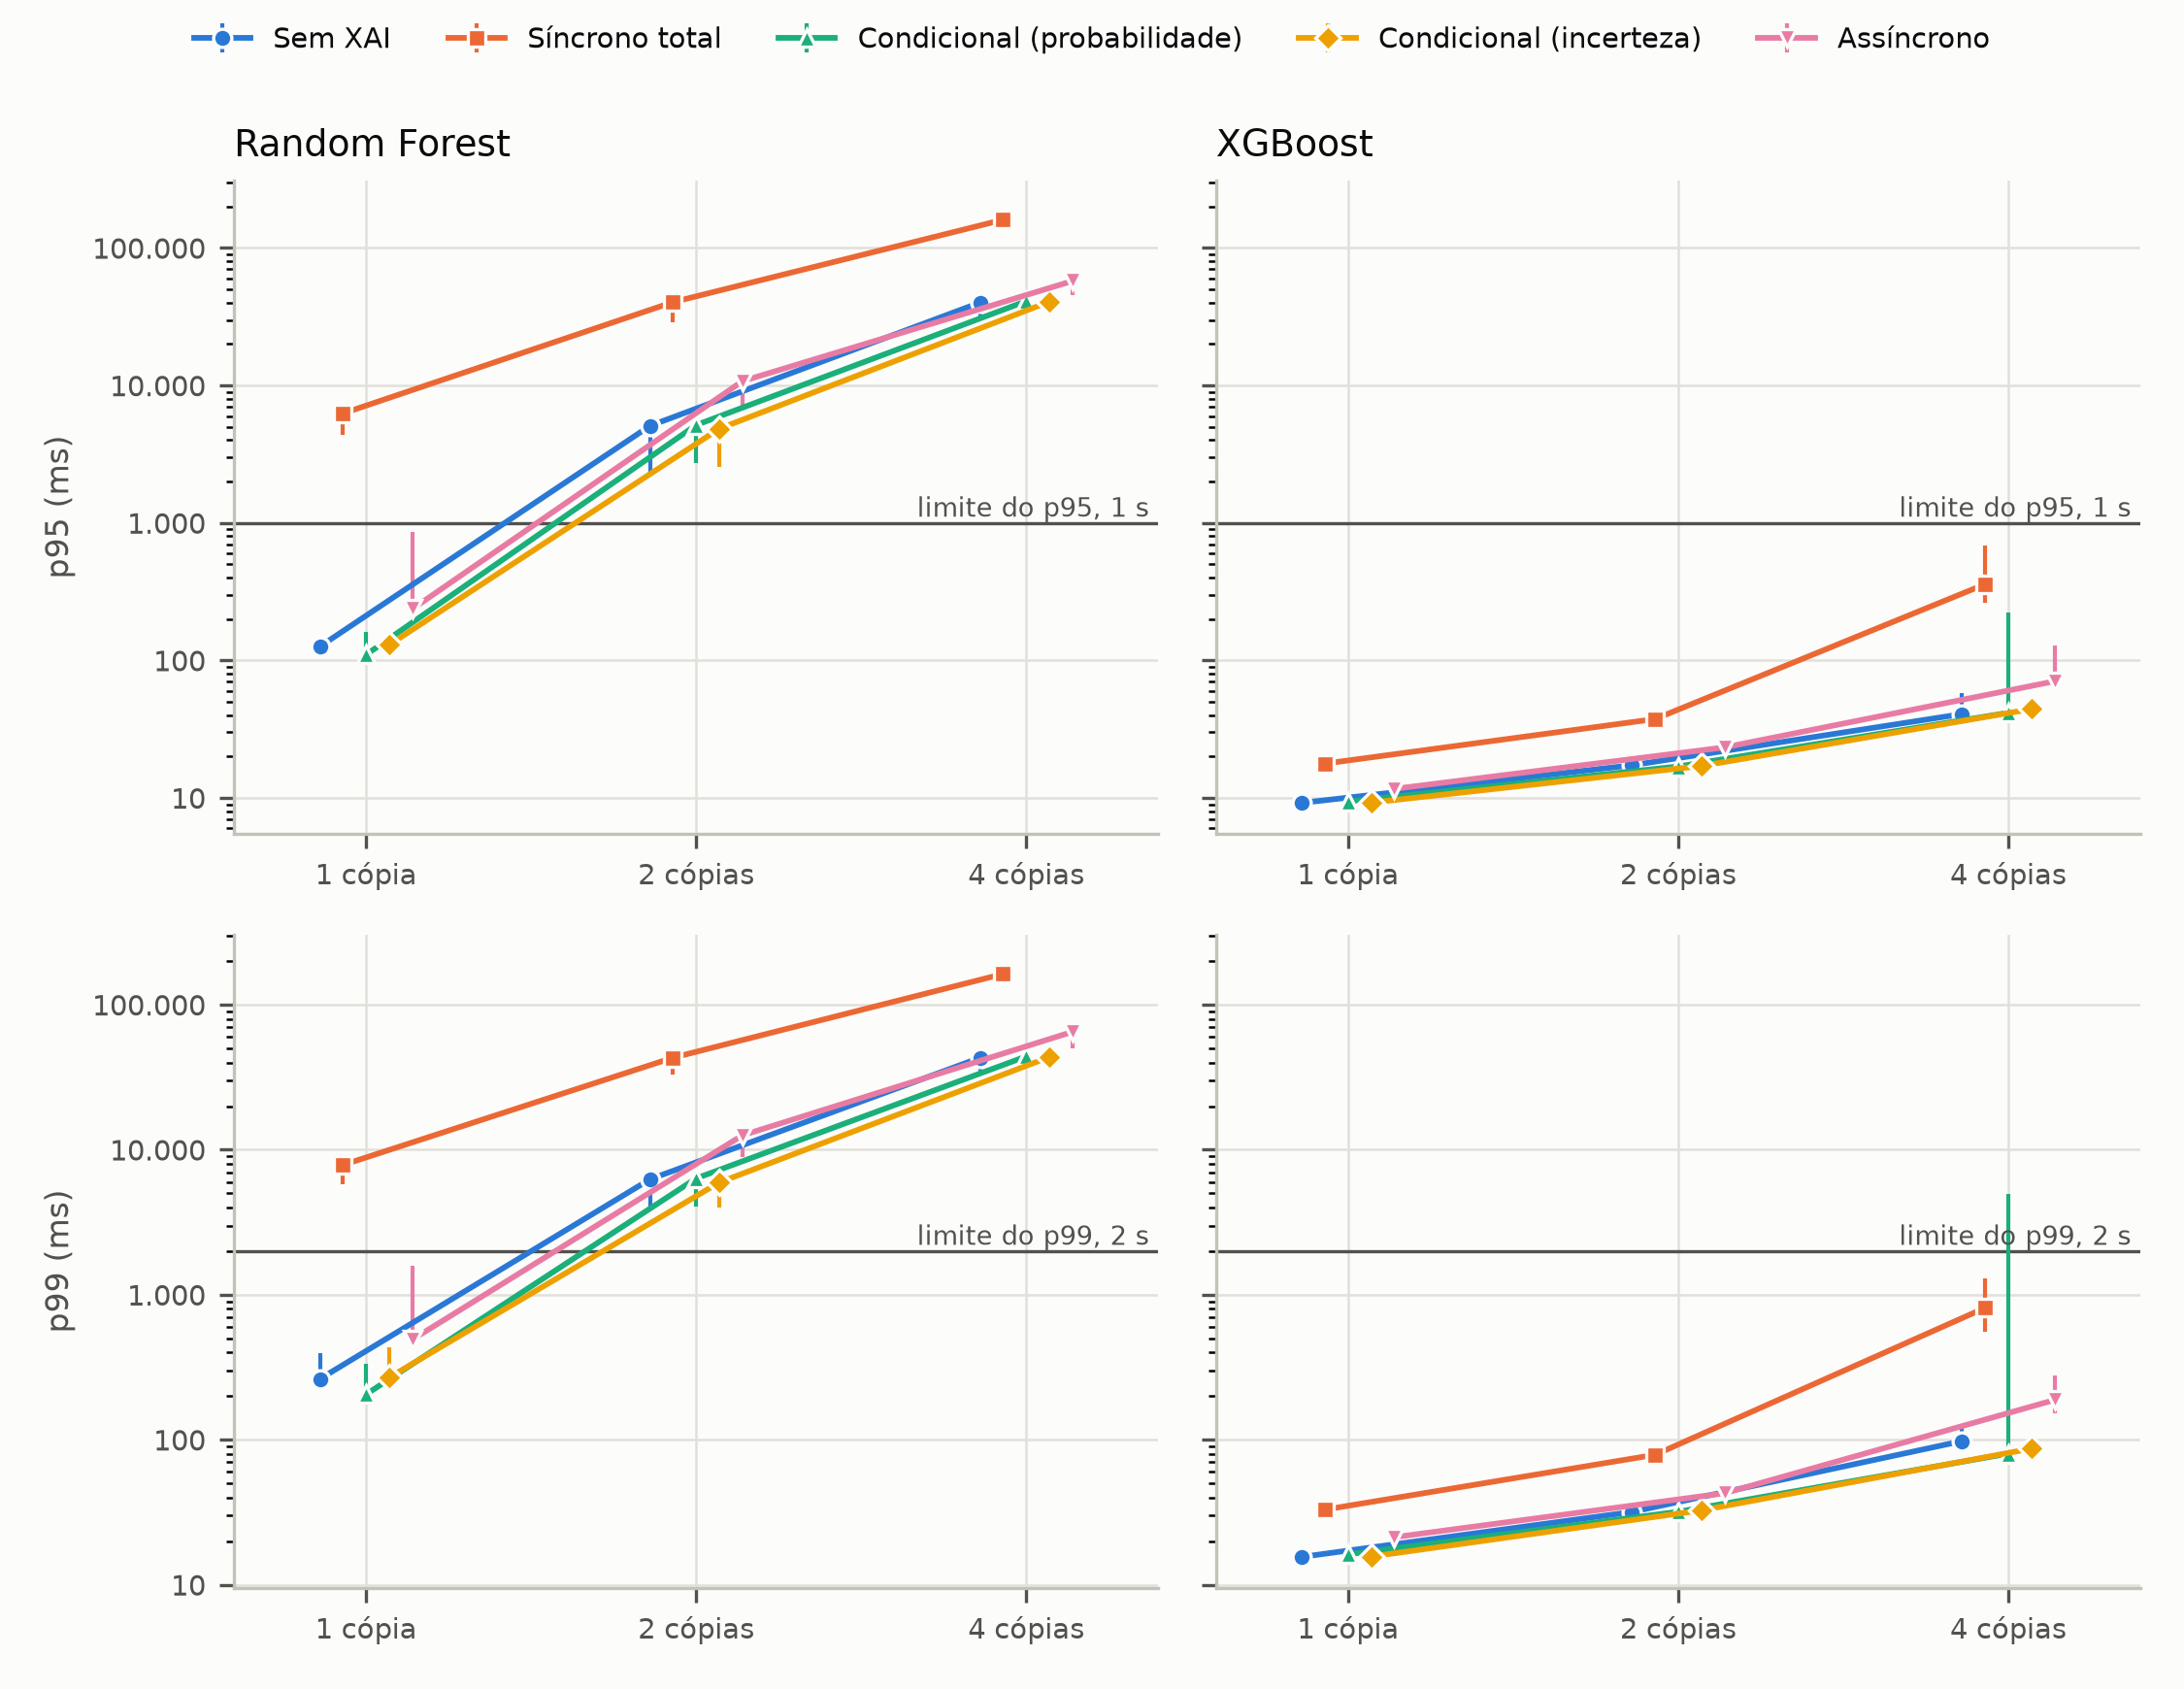
\includegraphics[width=\textwidth]{figuras/latencia-classificacao.png}
  \fonte{Elaborada pelos autores.}
  \nota{Cada ponto é a mediana das 3 execuções, e a barra vai do mínimo ao máximo. As linhas
  horizontais marcam os limites de 1~s no p95 e de 2~s no p99. O eixo vertical é logarítmico.}
\end{figure}

\begin{table}[htbp]
  \centering
  \caption{p95 da latência de classificação, em milissegundos}
  \label{tab:latencia}
  \begin{tabular}{llrrr}
    \toprule
    Classificador & Configuração & 1 cópia & 2 cópias & 4 cópias \\
    \midrule
    Random Forest & Sem XAI & 126,2 & 5.086* & 40.103* \\
    & Síncrono total & 6.265* & 40.413* & 160.610* \\
    & Condicional, probabilidade & 110,1 & 5.155* & 41.105* \\
    & Condicional, incerteza & 129,9 & 4.849* & 40.685* \\
    & Assíncrono & 236,6 & 10.751* & 57.541* \\
    \midrule
    XGBoost & Sem XAI & 9,2 & 17,3 & 40,8 \\
    & Síncrono total & 17,8 & 37,5 & 358,7 \\
    & Condicional, probabilidade & 9,4 & 16,9 & 41,6* \\
    & Condicional, incerteza & 9,2 & 17,1 & 44,3 \\
    & Assíncrono & 11,6 & 23,3 & 70,5 \\
    \bottomrule
  \end{tabular}
  \fonte{Elaborada pelos autores.}
  \nota{Mediana das 3 execuções de cada combinação. O asterisco marca as combinações inviáveis.}
\end{table}

A Figura~\ref{fig:pendentes} mostra o maior número de fluxos pendentes de classificação a cada
10~s, na repetição 1 do Sem XAI, do Síncrono total e do Assíncrono. No XGBoost, o maior número de
fluxos pendentes de uma execução ficou entre 63 e 865. No Random Forest, ele foi de 790 a 3.116 com
2 cópias e de 5.580 a 10.100 com 4 cópias. No Síncrono total com 4 cópias, os fluxos pendentes não
chegaram a zero em 99\% da execução.

\begin{figure}[htbp]
  \centering
  \caption{Fluxos pendentes de classificação ao longo da execução}
  \label{fig:pendentes}
  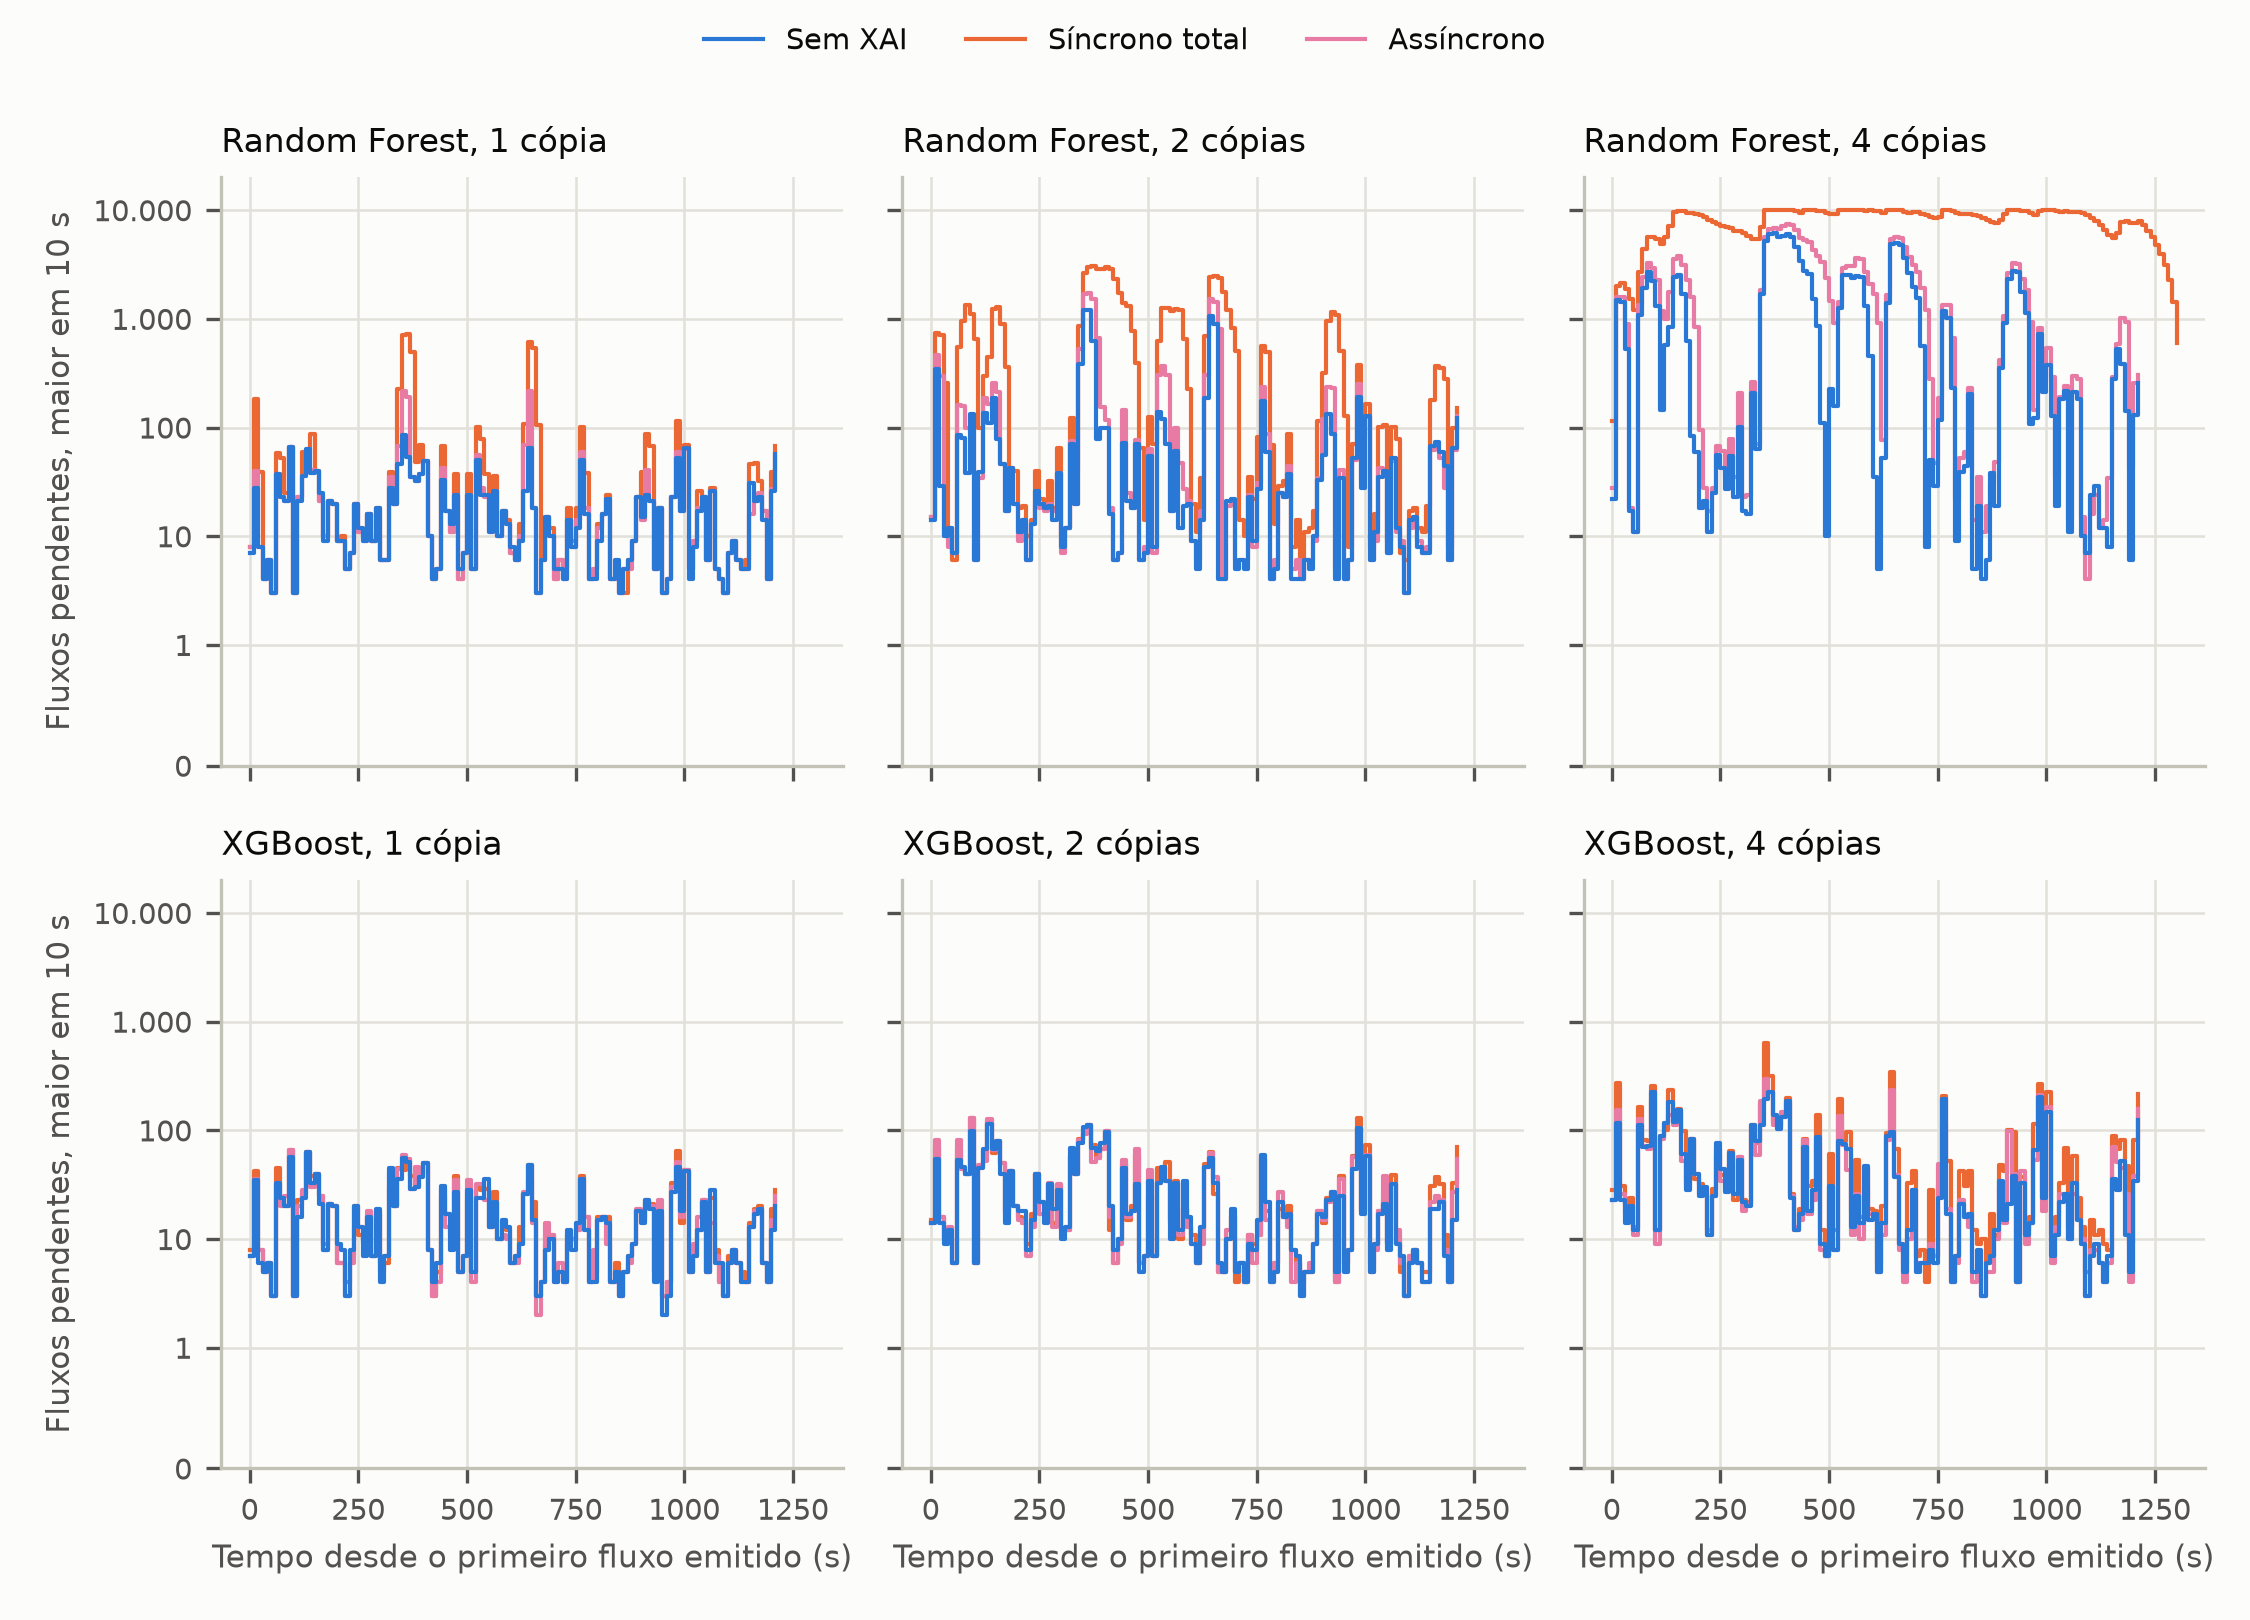
\includegraphics[width=\textwidth]{figuras/pendentes-classificacao.png}
  \fonte{Elaborada pelos autores.}
  \nota{Maior número de fluxos pendentes a cada 10~s, na repetição 1 de cada configuração. O eixo
  vertical é linear entre 0 e 1 e logarítmico acima de 1.}
\end{figure}

\subsection{Explicações: latência, fila e cobertura}

A Tabela~\ref{tab:explicacoes} traz o p95 da latência de explicação e a cobertura explicativa de
cada configuração que explica fluxos. No Síncrono total, a explicação fica disponível junto com a
classificação, e as duas latências coincidem. No Assíncrono do XGBoost, o p95 da latência de
explicação ficou menos de 2~ms acima do p95 da latência de classificação, nas três cargas.

A Figura~\ref{fig:fila} mostra o tamanho da fila de explicações pendentes nas execuções do
Assíncrono. No XGBoost, a fila teve no máximo 30 solicitações. No Random Forest, ela cresceu nas
rajadas de emissão, chegou a 1.869 a 2.085 solicitações com 2 cópias e atingiu o limite de 10.000
com 4 cópias, quando o NIDS descartou de 539 a 5.051 solicitações por execução. Em todas as
execuções do Assíncrono, o processo explicador concluiu as solicitações aceitas, nenhuma ficou
pendente, e a última explicação ficou disponível até 10,0~s depois da última solicitação, bem abaixo
do tempo máximo de esvaziamento de 300~s.

\begin{table}[htbp]
  \centering
  \caption{p95 da latência de explicação, em milissegundos, e fluxos explicados}
  \label{tab:explicacoes}
  \setlength{\tabcolsep}{4pt}
  \begin{tabular}{llrrrr}
    \toprule
    Classificador & Configuração & 1 cópia & 2 cópias & 4 cópias & Explicados (\%) \\
    \midrule
    Random Forest & Síncrono total & 6.265 & 40.413 & 160.610 & 100 \\
    & Condicional, probabilidade & 48,5 & 391,2 & 25.812 & 2,8 \\
    & Condicional, incerteza & 59,4 & 324,0 & 42.049 & 0,1 \\
    & Assíncrono & 1.636 & 23.318 & 157.421 & 100* \\
    \midrule
    XGBoost & Síncrono total & 17,8 & 37,5 & 358,7 & 100 \\
    & Condicional, probabilidade & 5,8 & 6,1 & 8,8 & 2,8 \\
    & Condicional, incerteza & 6,4 & 10,8 & 24,1 & 0,1 \\
    & Assíncrono & 13,3 & 24,9 & 72,1 & 100 \\
    \bottomrule
  \end{tabular}
  \fonte{Elaborada pelos autores.}
  \nota{Mediana das 3 execuções de cada combinação. Os explicados são a proporção dos fluxos
  classificados com a explicação concluída. *Com 4 cópias, a mediana foi de 95,9\%.}
\end{table}

\begin{figure}[htbp]
  \centering
  \caption{Fila de explicações pendentes ao longo da execução, no Assíncrono}
  \label{fig:fila}
  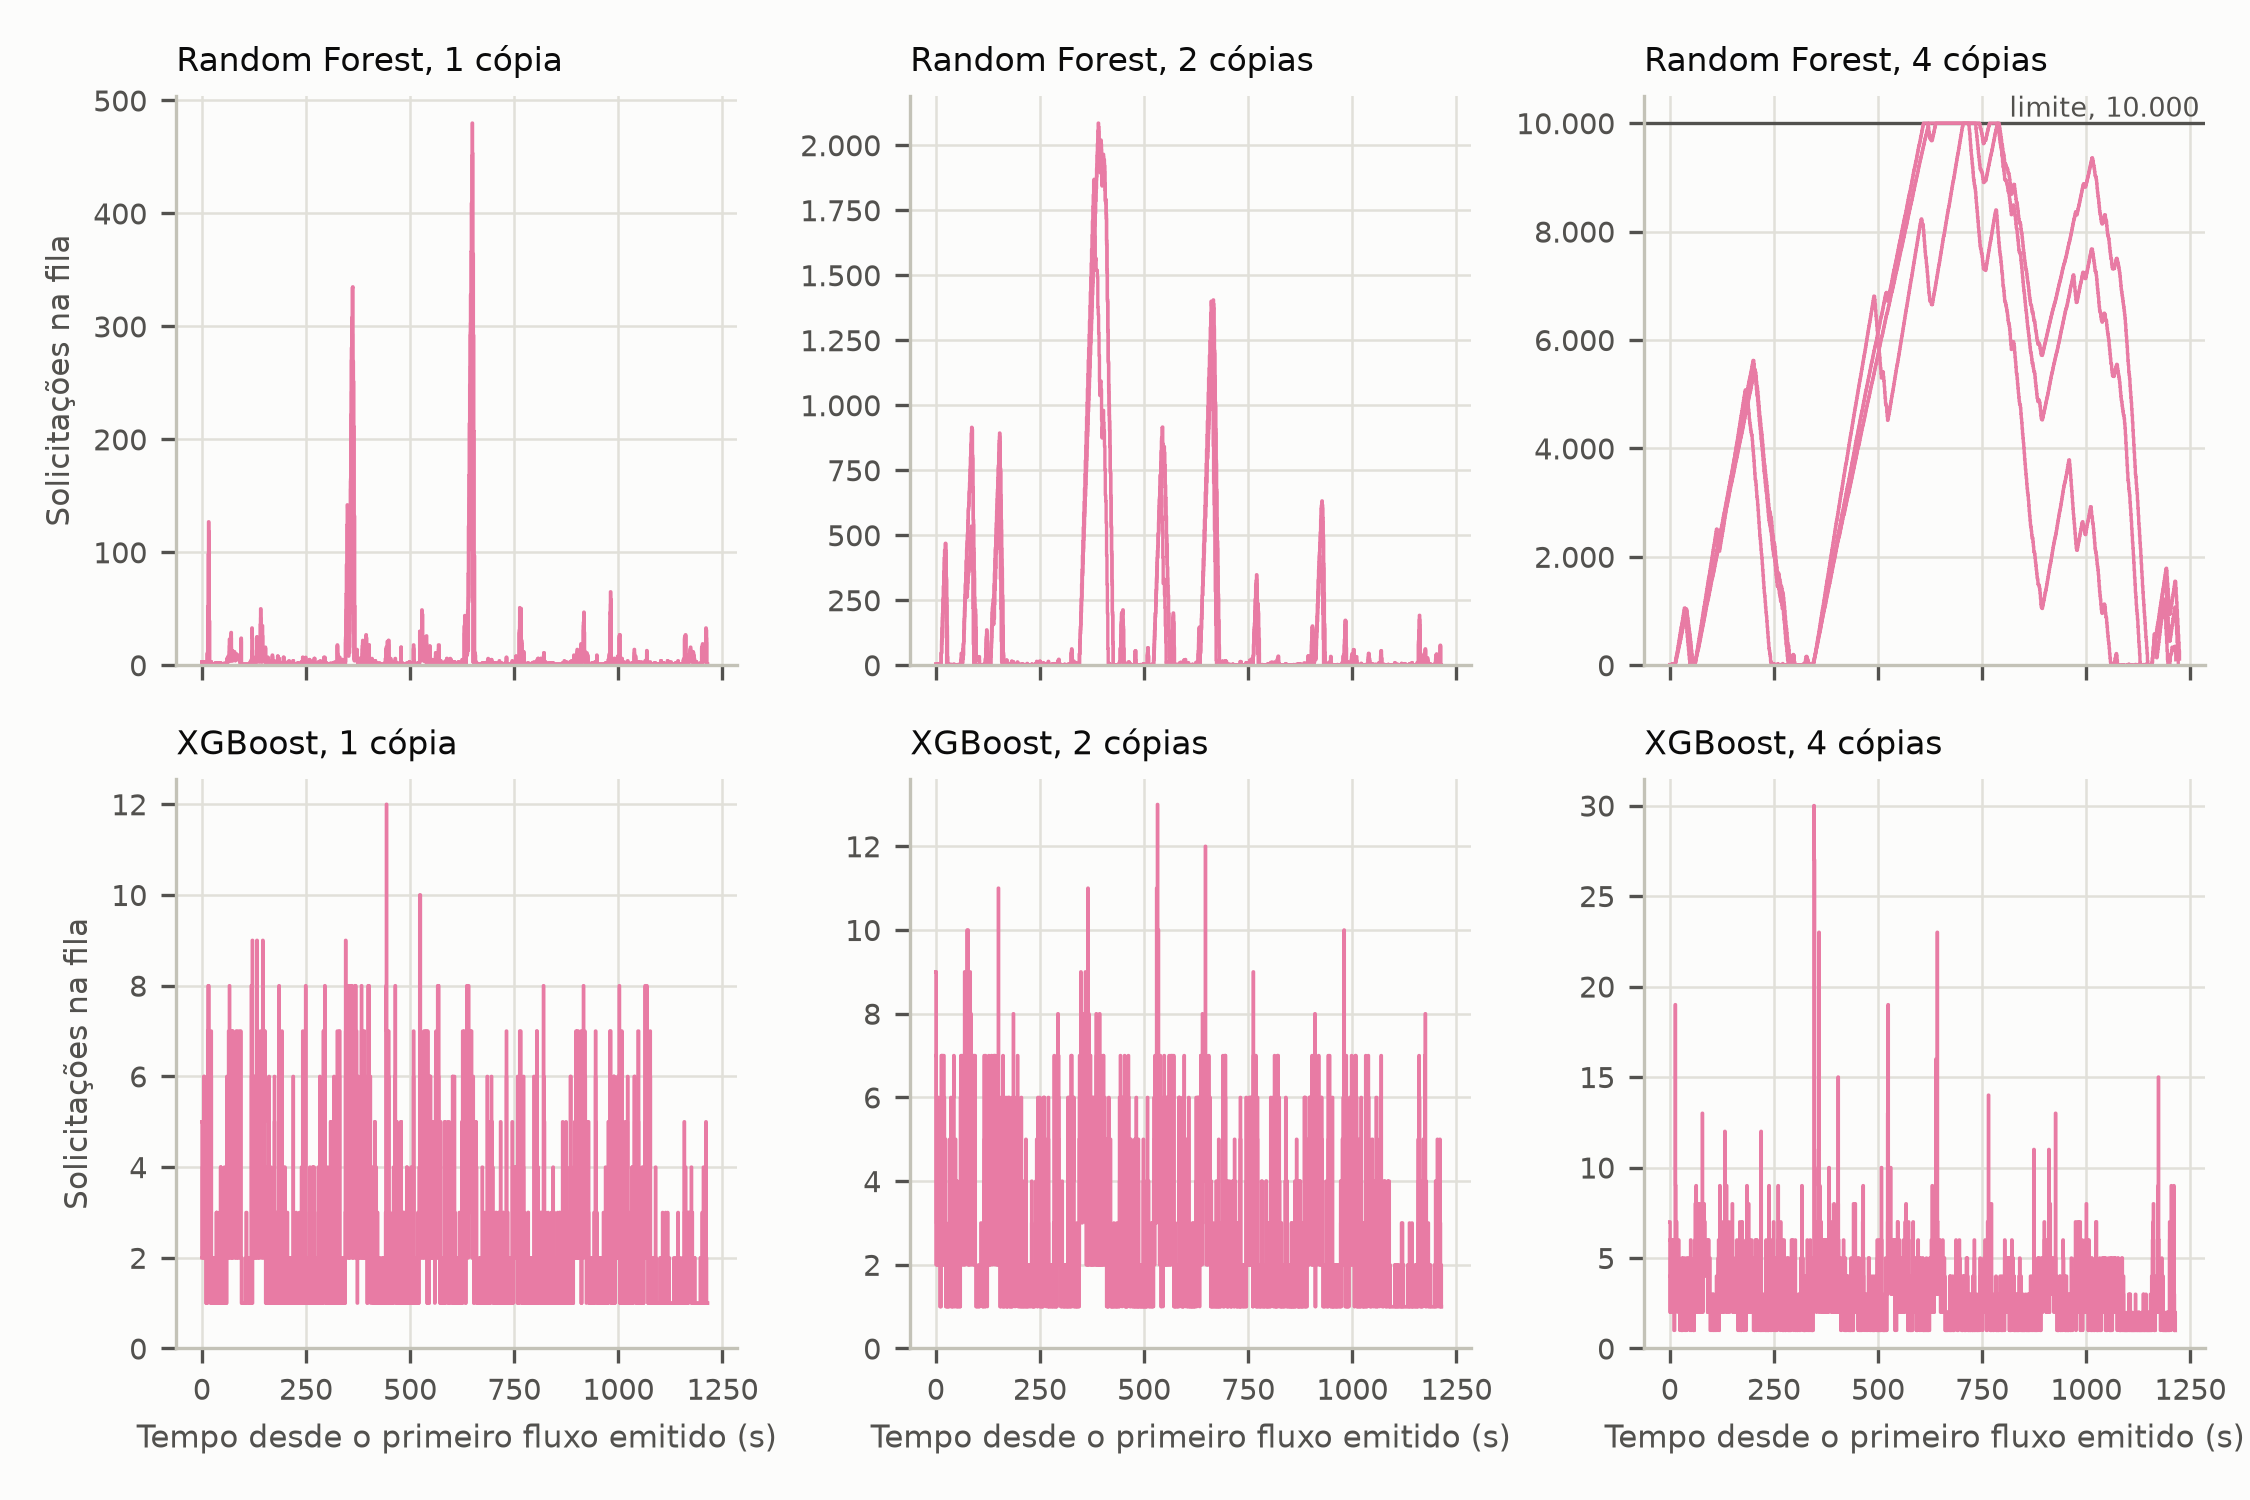
\includegraphics[width=\textwidth]{figuras/fila-explicacoes.png}
  \fonte{Elaborada pelos autores.}
  \nota{Maior tamanho da fila a cada segundo, nas 3 execuções de cada combinação.}
\end{figure}

\subsection{Uso de recursos}

A Tabela~\ref{tab:cpu} traz o tempo de CPU por fluxo classificado do classificador e do processo
explicador, com 1 e 4 cópias. O classificador é medido do início ao fim da captura, e o processo
explicador, do fim da carga do modelo ao fim do atendimento das solicitações. O tempo de CPU do
classificador por fluxo cresceu com a carga em todas as configurações, inclusive no Sem XAI, que
passou de 4,3~ms para 7,1~ms no Random Forest.

O pico de memória residente do classificador ficou entre 222 e 386~MiB, e o do processo explicador,
entre 201 e 204~MiB. O do extrator cresceu com o número de cópias, de 1.788 a 1.891~MiB com 1 cópia
para 4.912 a 4.981~MiB com 4, porque o extrator guarda os pacotes de cada fluxo e mantém cada fluxo
emitido até chegar outro pacote com a mesma chave.

\begin{table}[htbp]
  \centering
  \caption{Tempo de CPU por fluxo classificado, em milissegundos}
  \label{tab:cpu}
  \begin{tabular}{llrrrr}
    \toprule
    & & \multicolumn{2}{c}{Classificador} & \multicolumn{2}{c}{Processo explicador} \\
    Classificador & Configuração & 1 cópia & 4 cópias & 1 cópia & 4 cópias \\
    \midrule
    Random Forest & Sem XAI & 4,3 & 7,1 & --- & --- \\
    & Síncrono total & 11,7 & 14,8 & --- & --- \\
    & Condicional, probabilidade & 4,2 & 7,3 & --- & --- \\
    & Condicional, incerteza & 4,3 & 7,0 & --- & --- \\
    & Assíncrono & 4,7 & 8,7 & 6,8 & 11,7 \\
    \midrule
    XGBoost & Sem XAI & 0,70 & 0,79 & --- & --- \\
    & Síncrono total & 1,20 & 1,41 & --- & --- \\
    & Condicional, probabilidade & 0,74 & 0,81 & --- & --- \\
    & Condicional, incerteza & 0,70 & 0,86 & --- & --- \\
    & Assíncrono & 0,82 & 0,96 & 0,66 & 0,79 \\
    \bottomrule
  \end{tabular}
  \fonte{Elaborada pelos autores.}
  \nota{Mediana das 3 execuções de cada combinação. O processo explicador só existe no Assíncrono.}
\end{table}

\subsection{Viabilidade e discussão}
\label{sec:viabilidade}

Pelos critérios de viabilidade da Seção~\ref{sec:metodologia}, 18 das 30 combinações de
classificador, configuração de explicação e nível de carga foram viáveis. No XGBoost, as cinco
configurações foram viáveis com 1, 2 e 4 cópias, com uma exceção. O Síncrono condicional por probabilidade com 4 cópias
foi viável em 2 das 3 execuções, e a execução inviável é a que perdeu 10.231 pacotes na captura, com
p99 da latência de classificação de 5,0~s. No Random Forest, só houve combinações viáveis com 1
cópia, no Sem XAI, nos dois critérios do Síncrono condicional e no Assíncrono. O Síncrono total do
Random Forest não foi viável em nenhuma carga, e, a partir de 2 cópias, nenhuma configuração do Random
Forest foi viável, nem o Sem XAI.

Os resultados sustentam a primeira parte da hipótese. A sobrecarga de latência cresceu com a carga
no Síncrono total e no Assíncrono, nos dois classificadores. No p95 do XGBoost,
ela foi de 8,6, 20 e 318~ms no Síncrono total, com 1, 2 e 4 cópias, e de 2,4, 6,0 e 30~ms no
Assíncrono. No Random Forest com 1 cópia, o Síncrono total acrescentou 6,1~s ao p95, e o Assíncrono,
110~ms. Nessas duas estratégias, o intervalo entre o mínimo e o máximo das execuções ficou acima do
intervalo do Sem XAI em todas as combinações, na média, no p95 e no p99.

O Síncrono condicional reduziu a sobrecarga a ponto de ela não se distinguir do Sem XAI em nenhuma
combinação, porque os intervalos entre o mínimo e o máximo das execuções se sobrepuseram. Em troca,
ele explicou poucos fluxos. O critério de probabilidade explicou 2,8\% dos fluxos classificados, e o
de incerteza, cerca de 0,1\%. Como o critério de probabilidade explica os fluxos classificados como
ataque, a cobertura dele acompanha a proporção de fluxos de ataque do trecho, de cerca de 2,8\%.
Tolay (2026) observa essa dependência da prevalência no CICIoT2023. Uma política que explica todos os
ataques previstos e parte dos benignos economizou de 15\% a 23\% do trabalho de explicação num
conjunto de teste balanceado e de 1,7\% a 2,6\% no conjunto com a distribuição original, dominada
por ataques. Num tráfego com mais ataques, o critério de probabilidade explicaria mais fluxos, e o
custo dele se aproximaria do custo do Síncrono total. A campanha não mediu essa condição.

O Assíncrono tirou a explicação do caminho da classificação e manteve a cobertura de 100\% enquanto
a fila de explicações pendentes teve vaga (Tabela~\ref{tab:explicacoes} e Figura~\ref{fig:fila}). O
custo passou para a latência de explicação e para o processo explicador. No Random Forest com 1
cópia, a explicação chegou com p95 de 1,6~s, contra 237~ms da classificação, e, com 4 cópias, a fila
encheu e a cobertura caiu para 94,8\% a 99,4\%. No XGBoost, a explicação ficou disponível logo
depois da classificação.

Mesmo sem esperar a explicação, o Assíncrono elevou a latência de classificação. No Random Forest com
1 cópia, a média do tempo de inferência foi de 4,2~ms, contra 3,9~ms no Sem XAI, e o p95 da latência
de classificação passou de 126~ms para 237~ms. O processo explicador roda em outro núcleo de
desempenho, e o experimento não mede a causa dessa diferença. Uma explicação possível é a disputa
dos recursos que os núcleos compartilham, como a memória cache de último nível.

No Random Forest, o limite de latência veio antes da explicação. Com 2 cópias, o Sem XAI já passou de
1~s no p95, com 2,3 a 5,1~s. A carga média dessas execuções, de 40,7 fluxos por segundo, com 4,7~ms
por inferência, ocupa o classificador por cerca de 19\% do tempo, e houve fluxo pendente de
classificação em 21\% do tempo. Esses fluxos se acumularam nas rajadas de
emissão, quando o extrator chegou a emitir 508 fluxos num segundo, e o acúmulo se desfez entre as
rajadas. A inviabilidade veio da concentração da emissão nas rajadas, e não da carga média. Só o
Síncrono total com 4 cópias saturou o NIDS. Nele, um único intervalo com fluxo pendente cobriu 99\%
da execução, e o classificador só alcançou a emissão depois do fim do tráfego. Nessas
execuções, a fila de saída do extrator encheu, e o NIDS descartou de 11,7\% a 21,2\% dos fluxos.

O tempo de CPU mostra o mesmo compromisso (Tabela~\ref{tab:cpu}). No Random Forest com 1 cópia, o
classificador usou 11,7~ms de CPU por fluxo classificado no Síncrono total, contra 4,3~ms no Sem XAI.
No Assíncrono, o custo se dividiu entre 4,7~ms no classificador e 6,8~ms no processo explicador. O
Assíncrono não reduz o trabalho de explicar. Ele o leva para outro núcleo, que precisa estar livre
para isso.

A diferença entre os dois classificadores aparece também na medição de Tolay (2026), feita fora de
um NIDS, em lotes de 1 a 5.000 registros do CICIoT2023. Com lotes de 1 registro, o TreeSHAP levou
0,126~s no Random Forest e 0,0033~s no XGBoost. Os modelos e o processador diferem dos deste
trabalho, e os valores absolutos não se comparam, mas nos dois casos explicar o Random Forest custa
muito mais que explicar o XGBoost. Este trabalho acrescenta o efeito desse custo na entrega da
classificação sob carga. Com o XGBoost, explicar todos os fluxos antes de entregar a classificação
coube nos limites de latência até 4 cópias. Com o Random Forest, não coube nem com 1 cópia.

Nugraha, Jnanashree e Bauschert (2025) explicam um detector XGBoost com SHAP e LIME, relatam que o
arcabouço deles reduziu o tempo de explicação do LIME de 36~s para 4,9~s e concluem que detecção
precisa e interpretabilidade quase em tempo real podem coexistir. Os resultados do XGBoost são
compatíveis com essa conclusão para o TreeSHAP, com a latência medida na entrega da classificação. Le
et al. (2026) avaliam políticas que escolhem entre ações de explicação, como suprimir, adiar ou gerar
a explicação local completa, numa simulação com sequências de escores e custos de explicação
normalizados, sem medir latências num NIDS. A fila de explicações pendentes do Assíncrono do Random
Forest, que cresceu nas rajadas e encheu com 4 cópias, é o tipo de acúmulo que essas políticas
procuram controlar, e as medições deste trabalho dão valores medidos para os custos que elas tratam
como parâmetros.

\subsection{Limitações}
\label{sec:limitacoes}

Os resultados valem para as condições do experimento e não implicam equivalência com redes físicas
de produção nem garantia de tempo real estrito. A rede é emulada numa única máquina, que também
reproduz o tráfego, e o classificador roda em Python, com uma \emph{thread}. O tráfego é um trecho de
20 minutos de um único dia, cujos ataques são todos de FTP-Patator, de modo que o Síncrono condicional
por probabilidade explica uma pequena parte dos fluxos. As cópias do trecho começam juntas, e as
rajadas de fluxos das cópias coincidem, o que torna os picos de carga proporcionais ao número de
cópias. Com rajadas desencontradas, a mesma carga média teria picos menores, e o Random Forest, que
passou do limite de latência pelo acúmulo de fluxos nas rajadas, poderia atender cargas maiores. A
campanha não mediu esse caso. Os fluxos das conexões anteriores ao início do trecho não correspondem
aos fluxos rotulados do dataset, embora façam parte da carga. Por fim, as latências medidas começam
no fim da extração dos atributos e não incluem a espera até a emissão do fluxo, que pode chegar a
120~s.

A carga também desacelera a máquina. Na campanha, a média do tempo de inferência do Random Forest no
Sem XAI, que não inclui nenhuma espera, subiu de 3,9~ms com 1 cópia para 6,4~ms com 4 cópias. A
mediana da frequência da CPU do classificador, lida a cada segundo, também subiu, de 400 a 523~MHz
com 1 cópia para 1.851 a 2.000~MHz com 4 cópias, mas a leitura de cada segundo não mostra a
frequência durante cada inferência. Os núcleos lógicos que dividem os núcleos físicos do
classificador e do processo explicador, que deveriam ficar ociosos, chegaram a 51\% a 100\% de
ocupação em algum segundo de cada execução. O experimento não separa as causas dessa queda, como a
disputa dos núcleos físicos e da memória com outros processos e o perfil de economia de energia
usado em todas as execuções. Parte da sobrecarga medida nas cargas maiores vem, assim, da máquina, e
não só do NIDS.

Cinco regras de análise foram fixadas depois da campanha, com os resultados já medidos. São a regra
que diz quando a fila de explicações pendentes cresce até o fim, a exigência de que as 3 execuções
de uma combinação sejam viáveis, o cálculo da sobrecarga pela diferença entre as medianas, o
critério de diferença entre combinações e a definição de saturação. Os limites de latência e de
descartes vieram do piloto, antes da campanha. Só duas conclusões dependem das regras fixadas
depois. O Síncrono condicional por probabilidade do XGBoost com 4 cópias seria viável se bastassem 2
das 3 execuções. A repetição 3 do Assíncrono do XGBoost com 4 cópias seria inviável por uma regra que
reprovasse a fila que volta, no último décimo da execução, ao maior tamanho que já tinha atingido.

Com 3 execuções por combinação, o trabalho não usa teste estatístico. Duas combinações são tratadas
como diferentes quando os intervalos entre o mínimo e o máximo das suas execuções não se sobrepõem,
um critério descritivo que não dá uma probabilidade de erro. Uma das execuções, do Síncrono
condicional por probabilidade do XGBoost com 4 cópias, perdeu 0,07\% dos pacotes na captura, e 1,2\%
dos fluxos dela ficaram com entradas diferentes das da leitura do arquivo. Pelos critérios de
validade, ela continua na análise.

\section{Considerações finais}
\label{sec:conclusao}

Este trabalho perguntou se é viável gerar explicações TreeSHAP no momento da classificação, num
NIDS baseado em aprendizado de máquina, sem violar as restrições de latência do tráfego. Nas
condições do experimento, a resposta depende do classificador. Com o XGBoost, foi viável em todas
as estratégias até 4 cópias do trecho, inclusive explicando todos os fluxos antes de entregar a
classificação, exceto numa execução que perdeu pacotes na captura. Com o Random Forest, explicar
todos os fluxos só foi viável fora do caminho da classificação, no Assíncrono, e com 1 cópia, a
única carga em que o próprio classificador sem explicação foi viável.

Cada estratégia troca uma vantagem por um custo. O Síncrono total explica todos os fluxos e soma o
tempo da explicação à latência de classificação, o que tornou o Síncrono total do Random Forest
inviável já com 1 cópia. O Síncrono condicional não acrescentou latência mensurável, mas explicou 2,8\% dos fluxos
pelo critério de probabilidade e cerca de 0,1\% pelo de incerteza, numa proporção que depende dos
ataques presentes no tráfego. O Assíncrono acrescentou menos latência de classificação que o
Síncrono total e explicou todos os fluxos enquanto a fila de explicações pendentes teve vaga, mas
atrasou as explicações, ocupou outro núcleo e, com 4 cópias no Random Forest, descartou solicitações.

Os resultados valem para uma única máquina, um trecho de 20 minutos de um único dia e cópias com
rajadas coincidentes (Seção~\ref{sec:limitacoes}). Trabalhos futuros podem medir as estratégias com
rajadas desencontradas e com tráfego de outros dias e ataques, que mudam a cobertura do critério de
probabilidade. Também podem separar as causas da queda de desempenho da máquina com a carga, com a
frequência dos núcleos fixa, e avaliar políticas que escolhem a ação de explicação conforme a fila,
como as de Le et al. (2026), com os custos medidos aqui.

% Referências manuais, em ordem alfabética, só com as fontes citadas.
\secaosemnumero{Referências}
\begingroup
\SingleSpacing
\setlength{\parindent}{0pt}
\setlength{\parskip}{\baselineskip}
\raggedright
ADADI, Amina; BERRADA, Mohammed. Peeking inside the black-box: a survey on explainable artificial
intelligence (XAI). \textbf{IEEE Access}, [\emph{s. l.}], v. 6, p. 52138--52160, 2018. DOI:
10.1109/ACCESS.2018.2870052.\par

APPNETA. \textbf{Tcpreplay}. Versão 4.6.2. [\emph{S. l.}]: GitHub, 2026. Disponível em:
\url{https://github.com/appneta/tcpreplay}. Acesso em: 17 nov. 2026.\par

BERTOLI, Gustavo de Carvalho \emph{et al.} Abordagem fim-a-fim para uso de aprendizado de máquina
em IDS: caso de detecção \emph{stateless} para TCP Scan. \emph{In}: SIMPÓSIO BRASILEIRO DE
SEGURANÇA DA INFORMAÇÃO E DE SISTEMAS COMPUTACIONAIS, 20., 2020, Petrópolis. \textbf{Anais}
[\ldots]. Porto Alegre: Sociedade Brasileira de Computação, 2020. p. 271--284. DOI: 10.5753/sbseg.2020.19243.\par

BREIMAN, Leo. Random forests. \textbf{Machine Learning}, [\emph{s. l.}], v. 45, n. 1, p. 5--32,
2001. DOI: 10.1023/A:1010933404324.\par

CHEN, Tianqi; GUESTRIN, Carlos. XGBoost: a scalable tree boosting system. \emph{In}: ACM SIGKDD
INTERNATIONAL CONFERENCE ON KNOWLEDGE DISCOVERY AND DATA MINING, 22., 2016, San Francisco.
\textbf{Proceedings} [\ldots]. New York: ACM, 2016. p. 785--794. DOI: 10.1145/2939672.2939785.\par

DASH, Sandhyarani; ACKEN, John M. Intrusion detection latency: the neglected metric.
\textbf{Cybersecurity}, [\emph{s. l.}], v. 9, n. 1, art. 144, 2026. DOI:
10.1186/s42400-026-00574-7.\par

ENGELEN, Gints. \textbf{CICFlowMeter}. Commit 13a061520b. [\emph{S. l.}]: GitHub, 2022. Disponível
em: \url{https://github.com/GintsEngelen/CICFlowMeter}. Acesso em: 17 nov. 2026.\par

ENGELEN, Gints. \textbf{CNS2022\_Code}. [\emph{S. l.}]: GitHub, 2023. Disponível em:
\url{https://github.com/GintsEngelen/CNS2022_Code}. Acesso em: 17 nov. 2026.\par

ENGELEN, Gints; RIMMER, Vera; JOOSEN, Wouter. Troubleshooting an intrusion detection dataset: the
CICIDS2017 case study. \emph{In}: IEEE SECURITY AND PRIVACY WORKSHOPS, 2021, San Francisco.
\textbf{Proceedings} [\ldots]. [\emph{S. l.}]: IEEE, 2021. p. 7--12. DOI:
10.1109/SPW53761.2021.00009.\par

GRINSZTAJN, Léo; OYALLON, Edouard; VAROQUAUX, Gaël. Why do tree-based models still outperform deep
learning on typical tabular data? \emph{In}: CONFERENCE ON NEURAL INFORMATION PROCESSING SYSTEMS,
36., 2022, New Orleans. \textbf{Advances in Neural Information Processing Systems 35}.
[\emph{S. l.}]: Neural Information Processing Systems Foundation, 2022. p. 507--520. DOI:
10.52202/068431-0037.\par

HENDRICKX, Kilian \emph{et al.} Machine learning with a reject option: a survey. \textbf{Machine
Learning}, [\emph{s. l.}], v. 113, n. 5, p. 3073--3110, 2024. DOI: 10.1007/s10994-024-06534-x.\par

LANTZ, Bob; HELLER, Brandon; MCKEOWN, Nick. A network in a laptop: rapid prototyping for
software-defined networks. \emph{In}: ACM SIGCOMM WORKSHOP ON HOT TOPICS IN NETWORKS, 9., 2010,
Monterey. \textbf{Proceedings} [\ldots]. New York: ACM, 2010. p. 1--6. DOI:
10.1145/1868447.1868466.\par

LE, Tran Duc \emph{et al.} Explanation-surface governance in
XAI-enabled network intrusion detection under resource constraints. \textbf{Research Square},
2026. Preprint, versão 1. DOI: 10.21203/rs.3.rs-9800570/v1.\par

LIU, Lisa \emph{et al.} Error prevalence in NIDS
datasets: a case study on CIC-IDS-2017 and CSE-CIC-IDS-2018. \emph{In}: IEEE CONFERENCE ON
COMMUNICATIONS AND NETWORK SECURITY, 2022, Austin. \textbf{Proceedings} [\ldots]. [\emph{S. l.}]:
IEEE, 2022. p. 254--262. DOI: 10.1109/CNS56114.2022.9947235.\par

LUNDBERG, Scott M.; LEE, Su-In. A unified approach to interpreting model predictions. \emph{In}:
CONFERENCE ON NEURAL INFORMATION PROCESSING SYSTEMS, 31., 2017, Long Beach. \textbf{Advances in
Neural Information Processing Systems 30}. Red Hook: Curran Associates, 2017. p. 4765--4774.\par

LUNDBERG, Scott M. \emph{et al.} From local explanations to global understanding with explainable
AI for trees. \textbf{Nature Machine Intelligence}, [\emph{s. l.}], v. 2, n. 1, p. 56--67, 2020.
DOI: 10.1038/s42256-019-0138-9.\par

NUGRAHA, Beny; JNANASHREE, Abhishek Venkatesh; BAUSCHERT, Thomas. A versatile XAI-based framework
for efficient and explainable intrusion detection systems. \textbf{Annals of Telecommunications},
[\emph{s. l.}], v. 80, n. 11-12, p. 1095--1120, 2025. DOI: 10.1007/s12243-025-01118-9.\par

OGUNSEYI, Taiwo Blessing \emph{et al.} Performance analysis of explainable deep learning-based
intrusion detection systems for IoT networks: a systematic review. \textbf{Sensors},
[\emph{s. l.}], v. 26, n. 2, art. 363, 2026. DOI: 10.3390/s26020363.\par

SHAP. \textbf{shap}. Versão 0.54.1. [\emph{S. l.}]: GitHub, 2026. Disponível em:
\url{https://github.com/shap/shap}. Acesso em: 17 nov. 2026.\par

SHAPLEY, Lloyd S. A value for n-person games. \emph{In}: KUHN, Harold W.; TUCKER, Albert W. (ed.).
\textbf{Contributions to the theory of games}. Princeton: Princeton University Press, 1953. v. 2,
p. 307--318. DOI: 10.1515/9781400881970-018.\par

SHARAFALDIN, Iman; HABIBI LASHKARI, Arash; GHORBANI, Ali A. Toward generating a new intrusion
detection dataset and intrusion traffic characterization. \emph{In}: INTERNATIONAL CONFERENCE ON
INFORMATION SYSTEMS SECURITY AND PRIVACY, 4., 2018, Funchal. \textbf{Proceedings} [\ldots].
[\emph{S. l.}]: SciTePress, 2018. p. 108--116. DOI: 10.5220/0006639801080116.\par

SHWARTZ-ZIV, Ravid; ARMON, Amitai. Tabular data: deep learning is not all you need.
\textbf{Information Fusion}, [\emph{s. l.}], v. 81, p. 84--90, 2022. DOI:
10.1016/j.inffus.2021.11.011.\par

THE KERNEL DEVELOPMENT COMMUNITY. \textbf{Segmentation offloads}. Versão 7.4.0-rc3. [\emph{S. l.}]:
The Linux Kernel Documentation, [2026]. Disponível em:
\url{https://docs.kernel.org/networking/segmentation-offloads.html}. Acesso em: 19 nov. 2026.\par

TOLAY, Abdurrahman. Beyond detection accuracy: measuring explanation cost, stability, and utility
for resource-aware IoT intrusion detection. \textbf{arXiv}, 2026. Preprint 2608.10349v1. DOI:
10.48550/arXiv.2608.10349. Disponível em: \url{https://arxiv.org/abs/2608.10349}. Acesso em: 17
nov. 2026.\par

ZUECH, Richard; KHOSHGOFTAAR, Taghi M.; WALD, Randall. Intrusion detection and big heterogeneous
data: a survey. \textbf{Journal of Big Data}, [\emph{s. l.}], v. 2, n. 1, art. 3, 2015. DOI:
10.1186/s40537-015-0013-4.\par
\endgroup


% Elementos pós-textuais opcionais:
% \secaosemnumero{Agradecimentos}
% [Registrar contribuições e financiamento, quando houver.]
%
% \secaosemnumero{APÊNDICE A -- [Título]}
% [Material elaborado pelo próprio autor.]
%
% \secaosemnumero{ANEXO A -- [Título]}
% [Material de terceiros, com a devida referência.]

\end{document}
